\documentclass{sbthesis}
\usepackage{graphicx}
\usepackage{listings}
\usepackage{color} % color
\usepackage{amsmath}
\definecolor{listinggray}{gray}{0.9}

% \IncludeFig{caption}{label}{file}{scale}
\newcommand{\IncludeFig}[4]{
  \begin{figure}[h]
    \centering
    \includegraphics[scale=#4]{#3}
    \caption{#1}
    \label{#2}
  \end{figure}
}

% \Ccode{title}{label}{file}
\newcommand{\Ccode}[3]{
  \lstset{language=c}
  \lstset{basicstyle=\footnotesize}
  \lstset{backgroundcolor=\color{listinggray},rulecolor=\color{blue}}
  \lstset{linewidth=\textwidth, xleftmargin=0pt, xrightmargin=0pt}
  \lstset{commentstyle=\textit, stringstyle=\upshape,showspaces=false}
  \lstset{frame=tb}
  \lstinputlisting[caption={#1},label={#2}]{#3}
}

\newcommand{\Matlab}[3]{
  \lstset{language=matlab}
  \lstset{basicstyle=\footnotesize}
  \lstset{backgroundcolor=\color{listinggray},rulecolor=\color{blue}}
  \lstset{linewidth=\textwidth, xleftmargin=0pt, xrightmargin=0pt}
  \lstset{commentstyle=\textit, stringstyle=\upshape,showspaces=false}
  \lstset{frame=tb}
  \lstinputlisting[caption={#1},label={#2}]{#3}
}

\title{A New Phantom and Gradient Isocenter Estimation for MRI Distortion Correction}
\author{Zongqi Cai}
\Department
\EmailAddress{caiz@csusb.edu}
\Advisor{Keith Evan Schubert}
\Committee*{Kay Zemoudeh}{Haiyan Qiao}{Reinhard Schulte}{}
\CSUSBDate{July 2013}
\Copyright

\AbstractText{abstract contents}
\AcknowledgementText{}
\DedicationText{To Zel and Septimus.}

\NoTables
\NoFigures

\begin{document}
\Thesis

\Chapter{Introduction}
\label{introduction}
\section{Thesis Overview}

Magnetic resonance imaging (MRI) provides an excellent modality for distinguishing different tissues 
in the human body, which makes 
this modality essential for medical applications. MRI can also be used for treatment planning of 
medical procedures that require a great degree of geometrical accuracy such as  
functional radiosurgery~\cite{Kond99}. Unfortunately, the accuracy of MRI for medical targeting applications 
is compromised by the presence of geometric distortions such as non-linearities of the magnetic gradient 
fields or inhomogeneities of the scanner main field 
~\cite{Dor05,LSS06a,LSS06b,LSS08a,LSS08b,Lang99,Wang04a,Wang04b}. 
Gradient nonlinearities can cause over 2mm of distortion to the location of features in the 
image~\cite{LSS08b,Lang99}.

Modern MRI scanners have built-in distortion correction algorithms, that rely on knowledge of the magnetic 
field configuration and its distortion. Built-in algorithms, which are usually proprietary, are designed 
based on assumed knowledge of the geometry and location of the gradient coils. A more practical approach is 
to use a phantom of known geometry and to derive the distortion by analyzing the MRI images generated with 
such a phantom ~\cite{Dor05,LSS06a,LSS06b,LSS08a,LSS08b,Lang99,Wang04a,Wang04b}. 
This method has the advantage that a scanner-specific correction can be applied, which can also take into 
account potential changes in the gradient fields over time.

Accurate knowledge of the gradient isocenter is essential to very accurate distortion correction methods, 
To our knowledge, existing distortion correction algorithms, both built-in and phantom based, 
make the assumption that the gradient isocenter coincides with the origin of the DICOM coordinates. 
This assumption may not be accurate and should not be used if a high degree of accuracy is necessary.

The goal of this work was to develop and implement a numerical software-based method to estimate the gradient 
isocenter of the magnetic field inside an MRI scanner using the MRI scan of a custom-built phantom.  
In our previous work~\cite{LSS06a,LSS06b,LSS08a,LSS08b}, we used an oil filled plexiglas cube with
159.50mm $\times$ 159.70mm $\times$ 158.11mm dimension that was designed to fit MR scanners that were 
available at that time.  Current MRI scanners have a significantly wider aperture, which necessitates 
a larger phantom to characterize the field distortion.  Furthermore, since the lower part of the scanner 
aperture is occupied by the scanner table, the scanning area occupied by the phantom or the patient is not 
centered on the gradient isocenter, making correction methods that assume that the phantom is centered with 
respect to the gradient isocenter~\cite{LSS06a,LSS06b,LSS08a,LSS08b,Lang99} obsolete and potentially 
inaccurate.

\begin{figure}[htb]
  \begin{minipage}{0.80\linewidth}
    \centering
    \centerline{\mbox{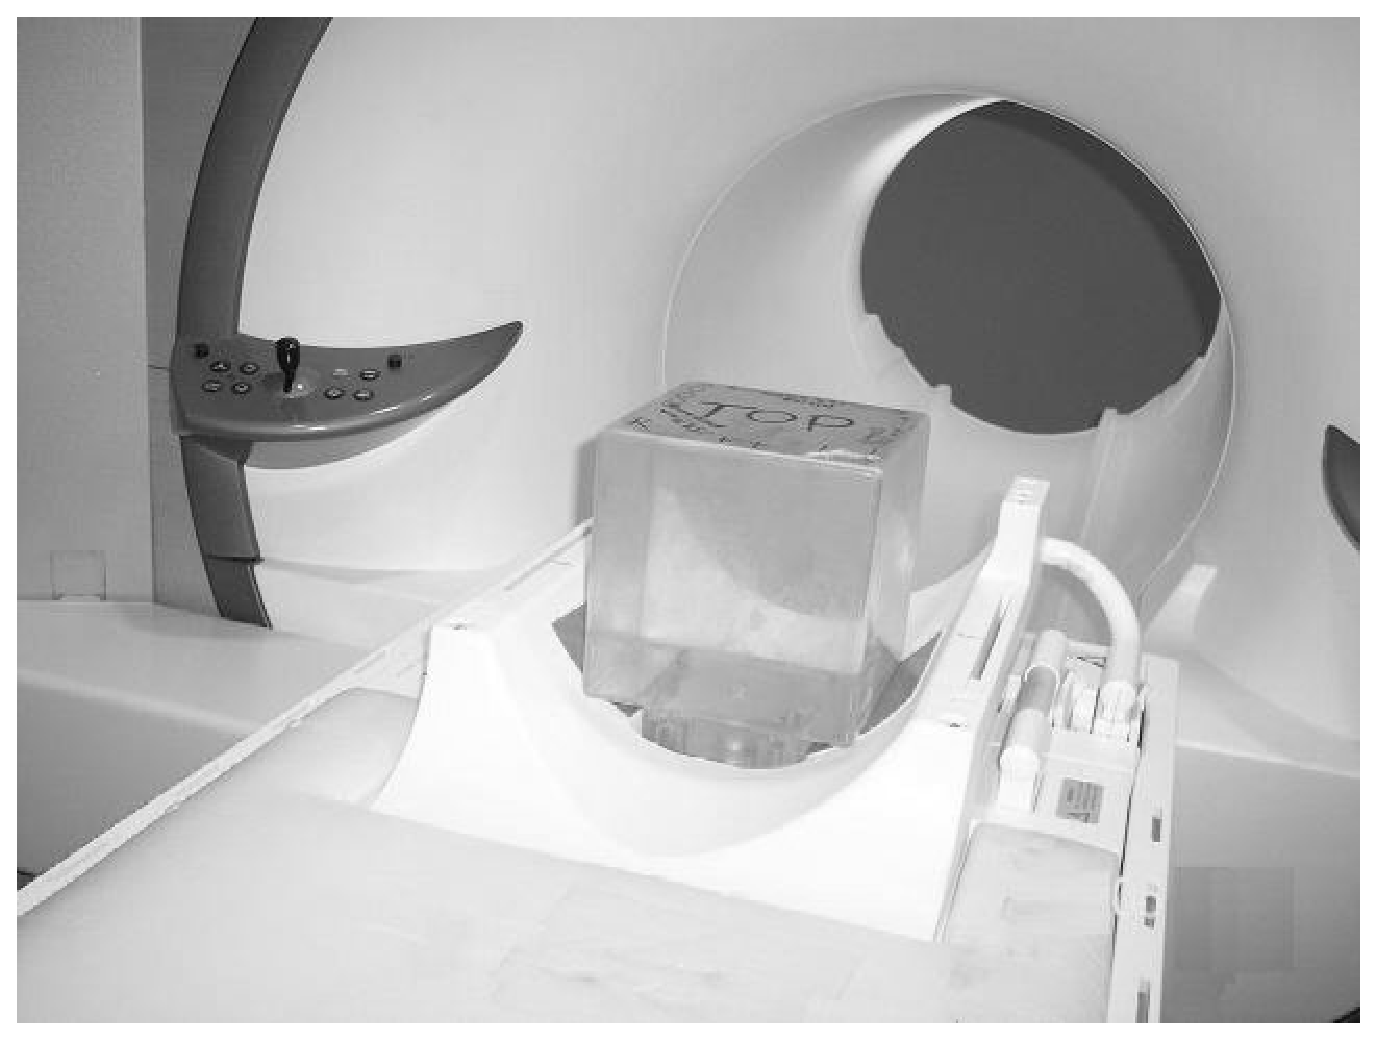
\includegraphics[width=4in]{introduction/images/phantom_scanner2.eps}}}
%    \centerline{New device}\medskip
    \centerline{}\medskip
  \end{minipage}
  \caption{A phantom cube made of plexiglas and filled with oil is ready for scanning} \label{fig:1}
\end{figure} 

The primary purpose of this thesis is to create method that would work in 3T MRI scanners as well as preivous
method in 1.5T scanners. To do this, we would need to addresss following issues in this work:
\begin{itemize}
\item A new phantom design that can capture the distortion in 3T MRI scanner. 
\item Algorithms that can extract interested data points from the MR images of the new phantom.
\item An algorithm that can accurately estimate the gradient ISO center of the magnetic field inside 3T MRI 
  scanners.
\item An algorithm that can accurately estimate the undistortion paramters which could then be used to generate
  undistorted images.
\end{itemize}

Thesis is going to start with the design details of the new phantom and several phases and changes we have
gone through. We will discuss some features captured by the final design of our phantom and their importance.

The next chapter will discuss the algorithm we derived to estimate the gradient ISO center using our unique
phantom design. Since there is no way to know the accurate location of ISO center inside MRI scanner, not even
the manufacture themselves, we will analyze our result using a simulate data points. 

After ISO center algorithm we will start to discuss a series of algorithms we used to extract data points
from MR images and CT images. CT images is used for measuring certain dimensions inside phantom due to
limitations of manufacture's macine. 

In the final chapter, putting everything together, 
we are using the geometric feature of the phantom and information
obtained from MR images to estimating a undistortion parameter that can transform the distorted MR images
back to undistorted images.

\section{Background}

The clinical application of protons was first suggested over 60 years ago \cite{Wil46}.
The ability to penetrate human tissue, delivering high dosage of proton beams at a target
region and being able to concentrate on a very small target area make protons ideal for use in noninvasive surgery \cite{Wil46}. Currently, Loma Linda University
Medical Center (LLUMC) is using proton beams to treat patients with tumors or
vascular malformations in the brain.
Due to the effectiveness of proton radiosurgery, a new system is proposed to treat
even smaller targets, more specifically, cranial targets.  However, this requires higher
accuracy of the treatment system. The current system can treat targets as small as 1 to 3 cm.  Target localization is accomplished using CT and projection angiography.
In order to achieve higher accuracy, MRI is to be used for target localization in the new
system. The major obstacle of using MRI is the gradient nonlinear
distortion on MRI images caused by the magnetic field of the scanner.
Two of the most important requirements for a successful distortion correction are:

\begin{enumerate}
\item The distortion correction must have submillimeter accuracy.
\item The correction process must be finished within 15 minutes.
\end{enumerate}

% I added some more detail in this paragraph

%The iteracy that this work is based on presented gradient nonlinearity correction method based on a cubic phantom MRI data set\cite{tom}.
This work is based on a published method for gradient nonlinearity correction using a cubic phantom MRI data set \cite{tom}. The published method utilizes the sum of spherical
harmonics to model the geometrically warped planes of the cube, and applies the model
to correct arbitrary image sets acquired with the same scanner. The cube is
placed in the MRI scanner such that the cube's center is exactly in the center of the MRI scanner.  This work assumes the center of the MRI scanner corresponds to the isocenter of the
magnetic field of the scanner. Opposite faces of the phantom are averaged, and three midplanes are fit to these surfaces.  Due to the symmetric property of the magnetic field,
the midplanes of different orientations of the phantom cube are undistorted.  Through each midplane, the ideal planes of different surfaces
of the cube are calculated simply by shifting the midplane to the direction
of the ideal plane by one-half the length of the cube. For each pixel on
the ideal plane, the sum of spherical
harmonics equation \ref{eq:spherical_harmonics} is applied to transform that pixel to the corresponding location on the distorted plane.

\begin{equation} \label{eq:spherical_harmonics}
\bar{\alpha} = \alpha(1 + K_{\alpha_0}(x^2 + y^2) + K_{\alpha_1}z^2 +
K_{\alpha_2}z^2(x^2 + y^2) + K_{\alpha_3}(x^2 + y^2)^2 +
K_{\alpha_4}z^4)
\end{equation}

Where $\bar{\alpha}$ and $\alpha$ are undistorted and distorted 3D coordinate respectively; $x$, $y$ and $z$ are coordinates of $\alpha$ on each axis; $K_{\alpha_i}$ are distortion parameters. Thus the distortion parameters in
equation \ref{eq:spherical_harmonics} are computed using linear least squares
technique.

Several assumptions are made for this model:
\begin{itemize}
  \item The phantom is (reasonably) centered with respect to the gradient isocenter of the scanner.
  \item The distortion is (reasonably) symmetric for each pair of faces.
  \item The origin of the DICOM patient coordinate system represents the position of the gradient isocenter.
\end{itemize}

However, positioning the phantom with respect to gradient isocenter is very difficult,
making it nearly impossible to perfectly center the phantom. After performing numerous
scans by Permedics Inc and LLUMC over the past several years, the issue of phantom centering has been identified
as a crucial factor in the quality of image data.  Improper centering of the phantom
in the scanner produces strong asymmetry in the phantom surfaces, thereby affecting the
accuracy of the distortion correction.  Therefore, the assumption that the distortion
is symmetric for each pair of phantom faces is invalid.

The assumption that the origin of the DICOM patient coordinate system corresponds to the isocenter of the magnetic field in the MRI scanner is also invalid. Siemens
engineers have confirmed that the true location of the gradient isocenter is unknown.
Investigating this further appeared to confirm this claim:  every scan performed thus far features a -10mm offset in Y in order to center the field of view on the phantom.  Therefore, the DICOM origin is shifted -10mm in $Y$ for each image.  But, the distortion inherent to each pair of phantom surfaces appears to be quite symmetric.  If the gradient isocenter was truly located at the DICOM origin, then the images would be expected to contain significant asymmetry in the distortion.  This is not the case in recent phantom studies.

In addition, the computation, including image filtering, distortion parameters
computation and final correction, average takes about 20-30 minutes.  In some cases, the calculation
could require as much as 40 minutes. This is far from the ideal 15 minutes requirement for clinical use.

\section{Significance}

% Which equation are you referring to here?  It would be better to reference the equation, instead of saying "the equation above"

Consider the minimization of the original expression for the sum of spherical harmonics:

\begin{equation} \label{eq:spherical_harmonics_2}
0 = \alpha(1 + K_{\alpha_0}(x^2_i + y^2_i) + K_{\alpha_1}z^2_i +
K_{\alpha_2}z^2_i(x^2_i + y^2_i) + K_{\alpha_3}(x^2_i + y^2_i)^2 +
K_{\alpha_4}z^4_i)
\end{equation}

The correction method this work proposes is on a pixel-to-pixel basis instead of a plane to plane basis.
Consider a point $P$ = $[X,Y,Z]$, where $X$, $Y$, and $Z$ are represented in equation \ref{eq:spherical_harmonics_2}. Each $X$, $Y$, and $Z$ describes the distance of $P$ from the DICOM origin (gradient isocenter), previously assumed to be at [0,0,0].  Past MRI studies have confirmed that the gradient isocenter is not at [0,0,0], therefore it is necessary to shift the DICOM origin appropriately by some offset $[\delta,\beta,\gamma]$.  Shifting the DICOM origin by this amount yields the new expression for $P$:

\begin{eqnarray}
P = [X - \delta, Y - \beta, Z - \gamma]
\end{eqnarray}

Substitute the new expression for $P$ into the sum of spherical harmonics expression:

$$0 = \alpha(1 + K_{\alpha_0}((x_i - \delta)^2 + (y_i - \beta)^2)$$
$$+ K_{\alpha_1}(z_i - \gamma)^2 + K_{\alpha_2}(z_i - \gamma)^2((x_i - \delta)^2 + (y_i - \beta)^2)$$
$$+ K_{\alpha_3}((x_i - \delta)^2 + (y_i - \beta)^2)^2 + K_{\alpha_4}(z_i - \gamma)^4)$$

Therefore, by expressing $P$ in this manner, the position of the true gradient isocenter becomes
$[\delta, \beta, \gamma]$. To solve for $\delta$, $\beta$, $\gamma$ and $K_{\alpha}$, we do not need
to have a full plane, as long as enough data points exist, and each data point exhibits a significant amount of distortion. The system can be solved using a linear least squares technique.

% To collect the data sets, a new phantom (Fig \ref{fig:2}), is proposed to capture data points on only the corner sections
% of the original phantom cube.  Since these sections are located far away from the gradient isocenter, they will exhibit the largest amount
% of distortion when compared to other sections closer to the gradient isocenter. The image slices that
% would be used are those close to each surface of the phantom. For each of these images a 
% filtering process will be applied to obtain only data points on the edge of phantom cube. 

% \begin{figure}[htb]
%   \begin{minipage}{0.80\linewidth}
%     \centering
%     \centerline{\mbox{\includegraphics[width=4in]{images/model2.eps}}}
% %    \centerline{New device}\medskip
%     \centerline{}\medskip
%   \end{minipage}
%   \caption{The new phantom, designed to collect data at the corners of the MRI scan.}  \label{fig:2}
% \end{figure}

% The reason for constructing a new phantom is that a phantom cube larger than original size (159.50 mm x 159.70 mm x 158.11 mm) is needed to 
% capture the distortion of larger MRI scanner while the manufacturer who produced the original
% phantom cube was having difficulty produce an accurate cubic phantom larger than the
% one shown in \ref{fig:1}. The eight parts, shown in fig \ref{fig:2}, will be interconnected and placed inside a water tank for scanning.
% For each image, eight curves representing the intersection between the surface of the material
% and water will be obtained, and will be used for calculating the gradient nonlinearity distortion correction.


\Chapter{Background}
\label{background}

% \Chapter{Overview}
% \label{overview}
% \input{overview/main}

% algorithm overviews
% canny, peakdet, steepest descent, dicom coordinate conversion etc

\Chapter{Phantom Design}
\label{phantom_design}
\section{Introduction}

Magnetic Resonance Imaging (MRI) provides an excellent modality for distinguishing different tissues in the
human body, which is essential for medical applications. When MRI is used for stereotactic treatment planning,
its geometric accuracy is crucial. Previous studies have been conducted to correct the distortion caused by
nonlinearity of the MRI scanner’s magnetic gradient fields by imaging a cubic phantom \cite{simple_approach},
\cite{tlee_iaeng} and defining
distortion correction functions based on the distorted appearance its surfaces. Correct mathematical handling
of the distortion correction function required that the cube was centered about the magnetic isocenter, which
is defined as the common center of the three magnetic gradient fields and  is not very accurately known.
New 3Tesla MRI systems have a larger bore, making the previous phantom design impractically small for probing
the field nonlinearity in the periphery of the bore, as the phantom cannot be scaled up due to constraints
related to weight and cost of manufacturing. We are introducing a new phantom design using a different
approach, which can be built to a larger size, improves accuracy of distortion characterization and reduces
cost.

\section{Initial Design}

The original phantom design, a 16-cm oil-filled cube, could not be scaled up due to weight and manufacturing
constraints. Our first modification was to look at changing the material to FR-4 since it is rigid, very flat,
and could be submerged for short periods of time to permit scanning the solid liquid interface in an MRI
machine.  Since most of the distortion is visible only in the corners, this was rapidly replaced by 8 corners
of a virtual cube, which could be connected by a rigid frame.  The weight of a tank to submerge either of
these designs to allow scanning was prohibitive, requiring a complete redesign.

\begin{figure}[htb]
  \begin{minipage}[t]{2.75in}
    \centering
    \centerline{\mbox{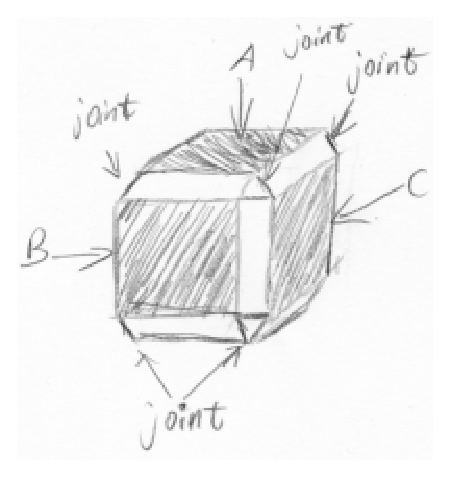
\includegraphics[width=2.75in]{phantom/images/brain_storm/model1.eps}}}
    \centerline{\emph{(a) First model}}
  \end{minipage}\medskip
  \begin{minipage}[t]{2.75in}
    \centering
    \centerline{\mbox{\includegraphics[width=2.75in]{phantom/images/brain_storm/model2.eps}}}
    \centerline{\emph{(b) Second model}}
  \end{minipage}
\end{figure}


\section{New Design}

The phantom is shaped to be as large as possible, while still fitting in the head coil of the scanner, so as
to achieve the maximum quality of signal and largest distortion. The phantom is an octagonal prism with 205mm
between opposite sides.  Each face of the octagonal prism is composed of 8 high precision NMR tubes that are
5mm in outer diameter and 205 mm in length. These tubes are filled with copper sulfate solution to generate a
strong signal in an MRI scanner.  The tubes are placed parallel to the magnetic field so they will cause less
susceptibility distortion \cite{mag_susceptibility},
and thus provide more accurate information on the gradient field.  In the
center of the phantom is a large water tank to help intensify the signals generated by the tubes. At one end
of the phantom is a cylindrical tank filled with copper sulfate, with a number of small solid cylinders in a
hexagonal pattern that are connecting the two surfaces of the tank. These cylinders are used to maintain the
long-term accuracy of the two surfaces, making sure they won’t deform, and are also aligned to the field to
minimize their effect on the field.  The data generated from 64 tubes mounted on the sides are designed to
give us x and y axis distortion information, and the end tank is designed to provide z-axis distortion data,
allowing a complete 3-D distortion correction with a relatively small amount of data.

\section{Sealing NMR Tubes}

Our original idea for sealing the NMR tubes was to use paraffin wax, either with or without a silicon seal.
Paraffin was heated and a liquid drop was then added to the tube as a seal , but had an uneven bottom caused
by the rapid solidifying of the wax, when it came in contact with the copper sulfate.  Additionally,
it tended to trap air bubbles, which made the end very hard to work with in the images.  Worst yet, after a
few weeks the liquid level in the tubes started to drop.  We decided to compare three potential alternatives:
machinable wax, water weld, and silicon sealer.  As the images on the right show, the silicon was far and
away the best.  There was no leakage lost, and since the setup time was slower on the liquid side it ended
up being almost completely flat.  Every feature was met, and it was also the most cost effective solution.

\begin{figure}[htb]
  \begin{minipage}[t]{1in}
    \centering
    \centerline{\mbox{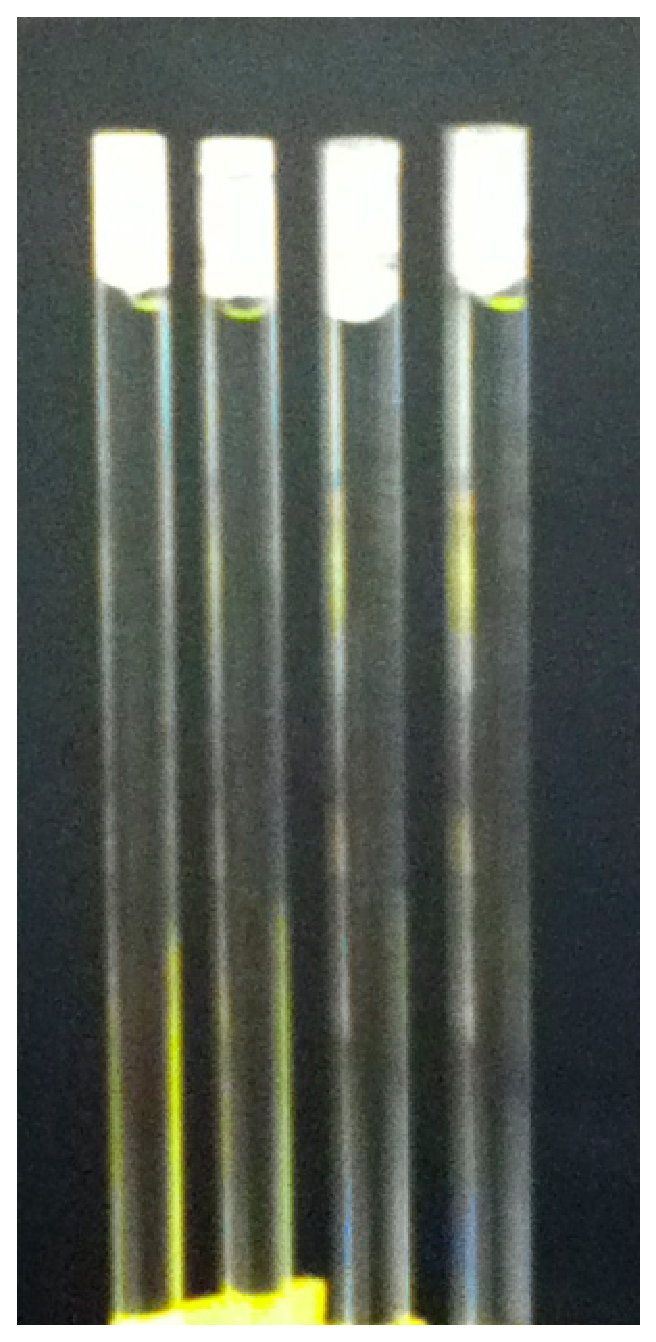
\includegraphics[width=1in]{phantom/images/tube_sealings/paraffin_and_floable_silicon.eps}}}
    \centerline{\emph{(a) Paraffin wax at top with floatable silicon at bottom}}
  \end{minipage}
  \begin{minipage}[t]{1in}
    \centering
    \centerline{\mbox{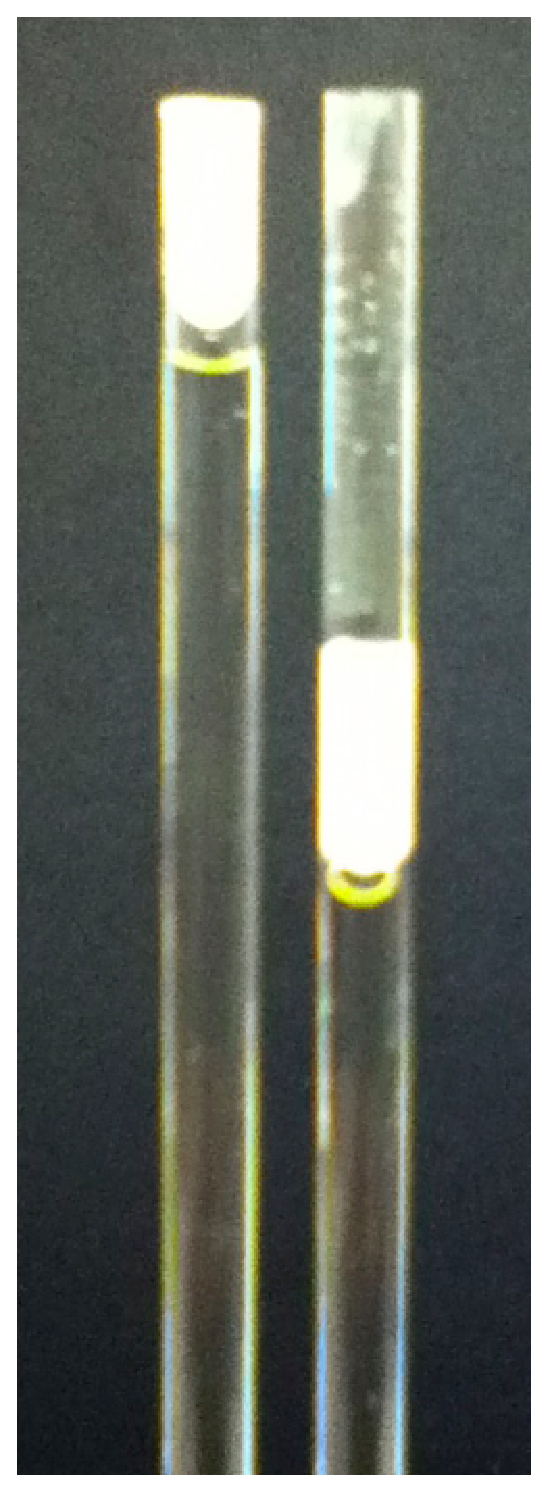
\includegraphics[width=1in]{phantom/images/tube_sealings/paraffin.eps}}}
    \centerline{\emph{(b) Paraffin wax only}}
  \end{minipage}

  \begin{minipage}[t]{1in}
    \centering
    \centerline{\mbox{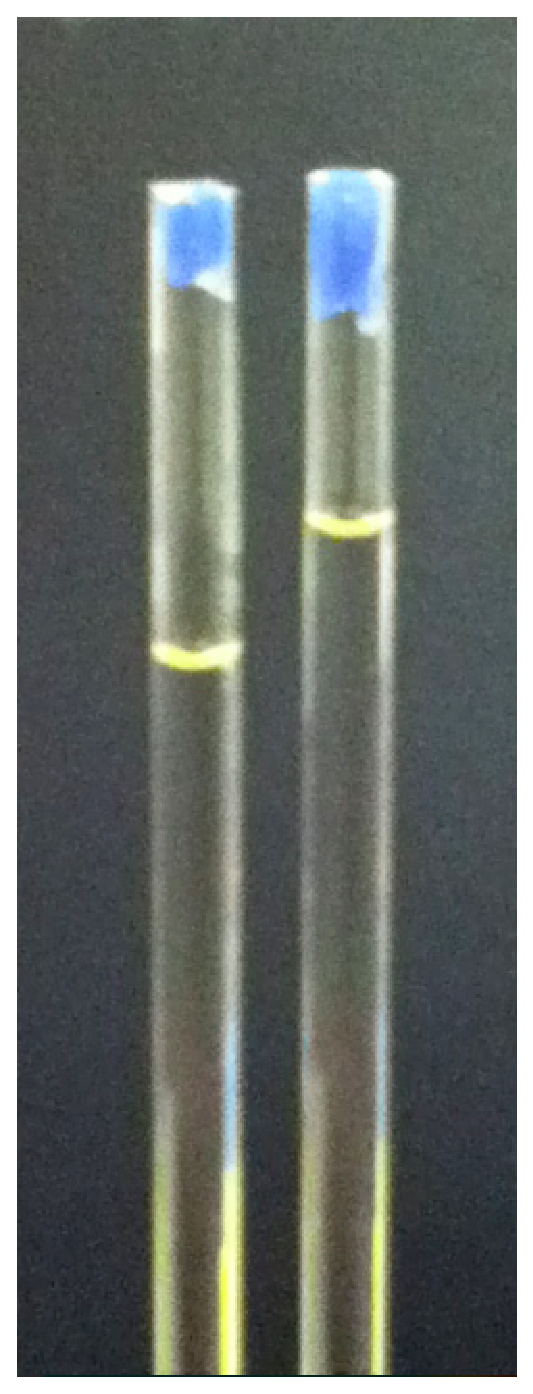
\includegraphics[width=1in]{phantom/images/tube_sealings/machinable_wax.eps}}}
    \centerline{\emph{(c) Machinable wax}}
  \end{minipage}\medskip
  \begin{minipage}[t]{1in}
    \centering
    \centerline{\mbox{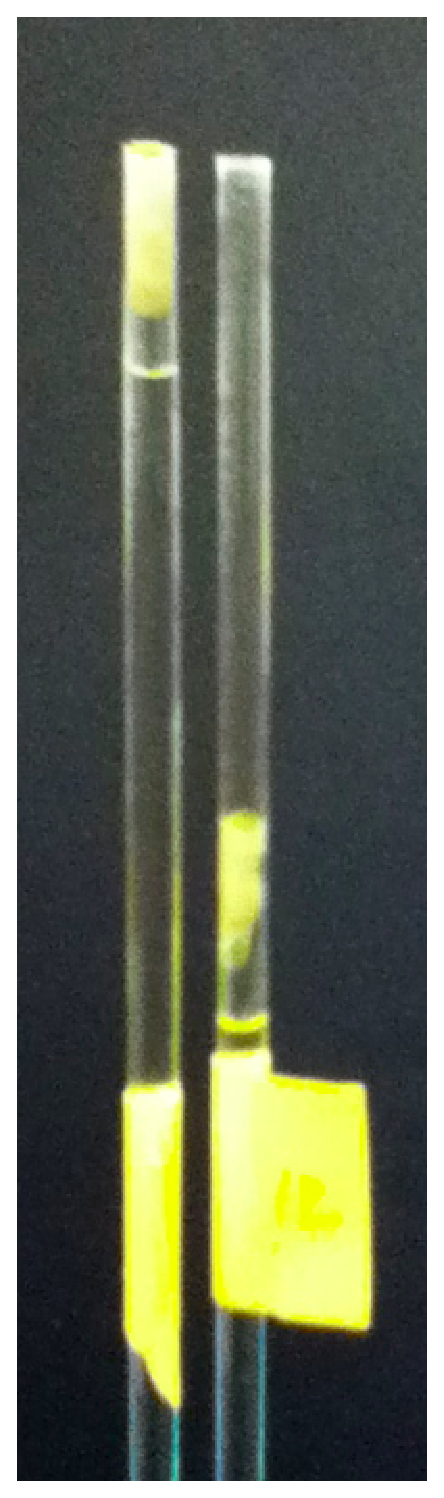
\includegraphics[width=1in]{phantom/images/tube_sealings/water_weld.eps}}}
    \centerline{\emph{(d) Water weld}}
  \end{minipage}

  \begin{minipage}[t]{1in}
    \centering
    \centerline{\mbox{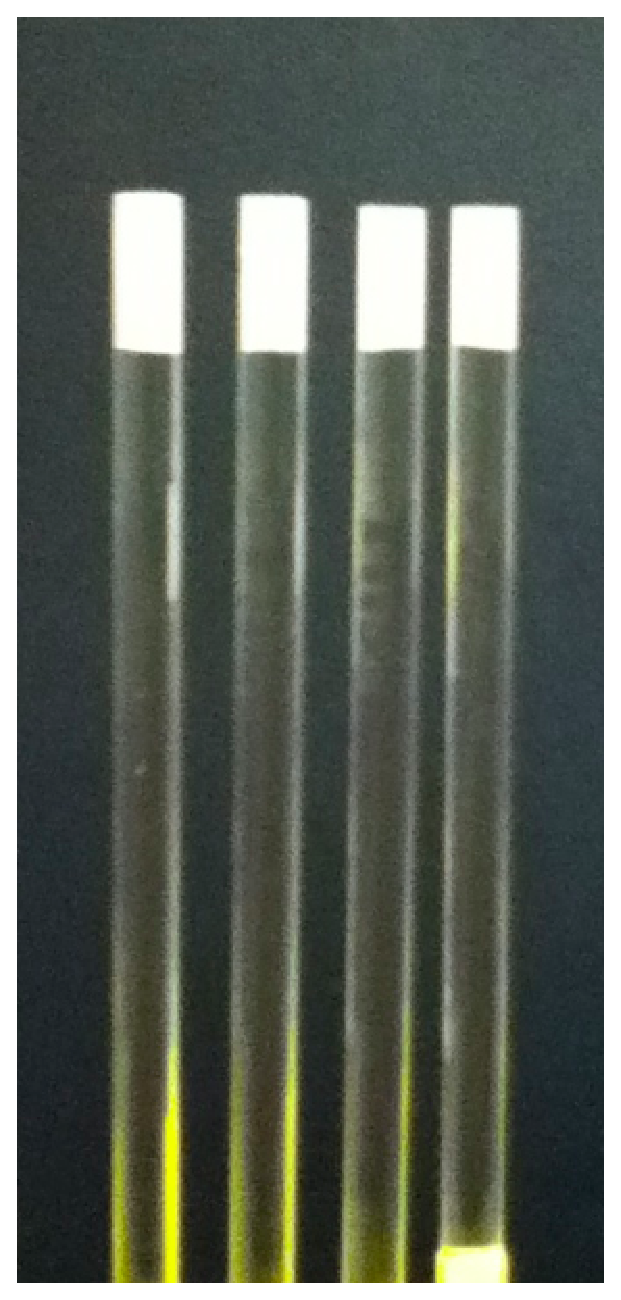
\includegraphics[width=1in]{phantom/images/tube_sealings/silicon.eps}}}
    \centerline{\emph{(e) Silicon}}
  \end{minipage}

\end{figure}

\section{Updated Desgin}

% \begin{figure}[htb]
%   \begin{minipage}[t]{1in}
%     \centering
%     \centerline{\mbox{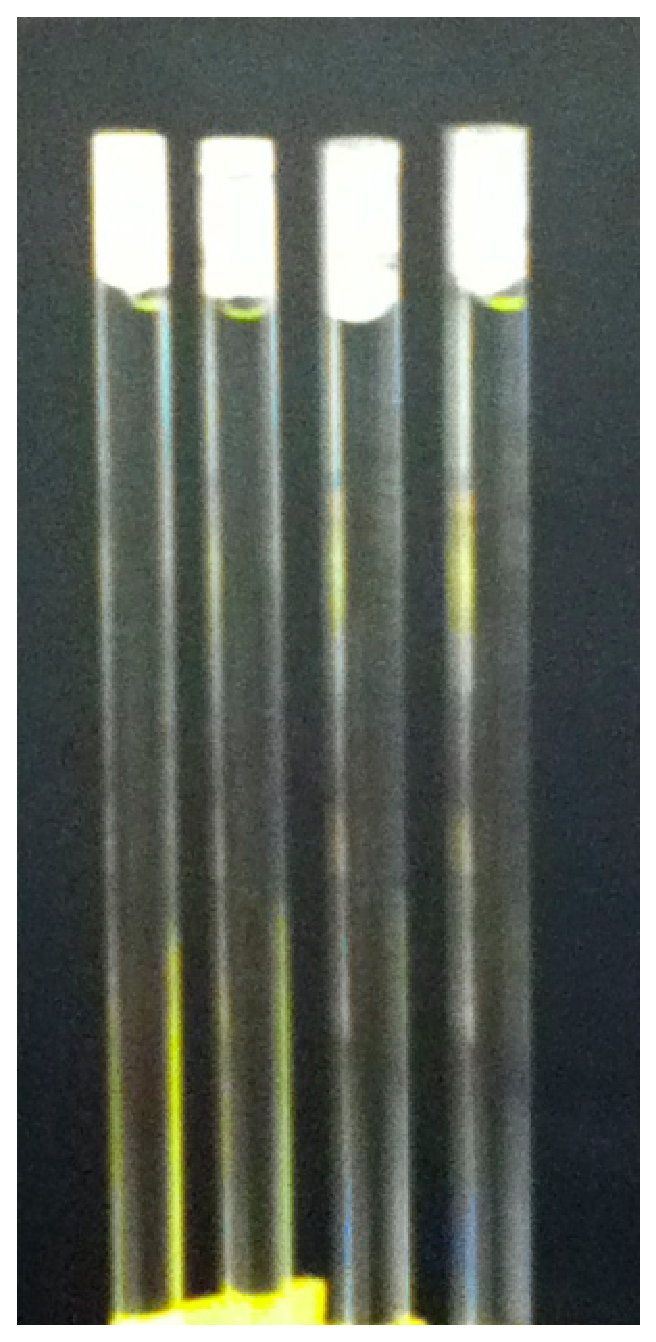
\includegraphics[width=1in]{phantom/images/tube_sealings/paraffin_and_floable_silicon.eps}}}
%     \centerline{\emph{(a) Paraffin wax at top with floatable silicon at bottom}}
%   \end{minipage}
%   \begin{minipage}[t]{1in}
%     \centering
%     \centerline{\mbox{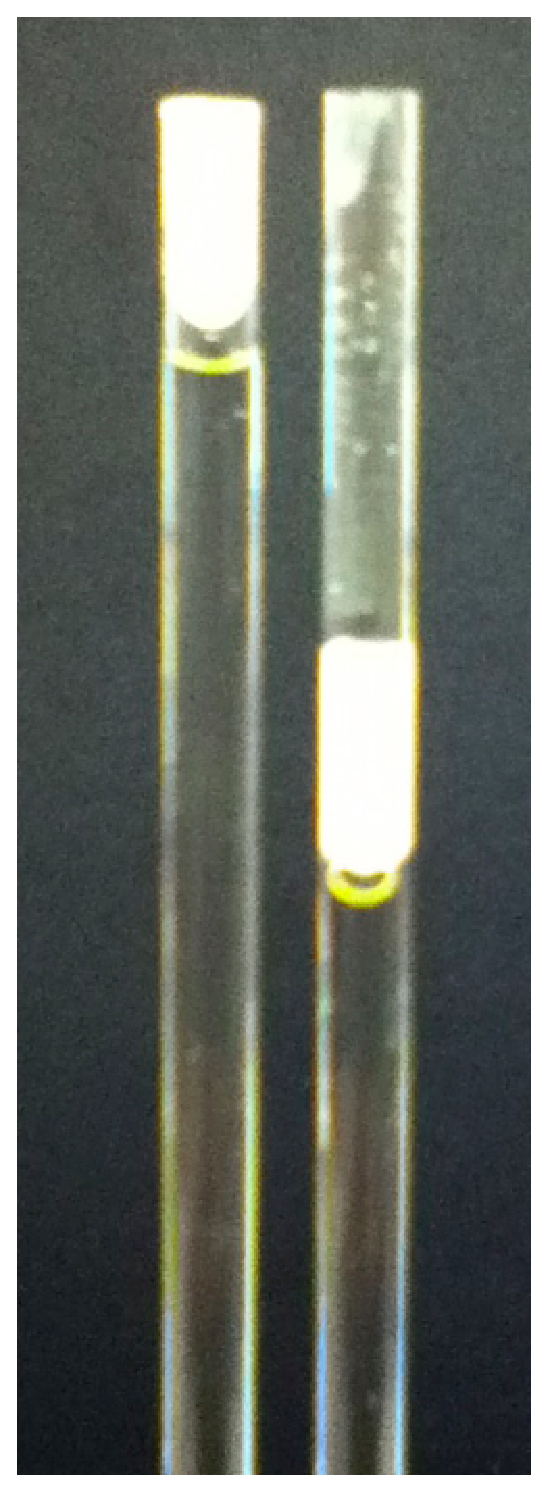
\includegraphics[width=1in]{phantom/images/tube_sealings/paraffin.eps}}}
%     \centerline{\emph{(b) Paraffin wax only}}
%   \end{minipage}

%   \begin{minipage}[t]{1in}
%     \centering
%     \centerline{\mbox{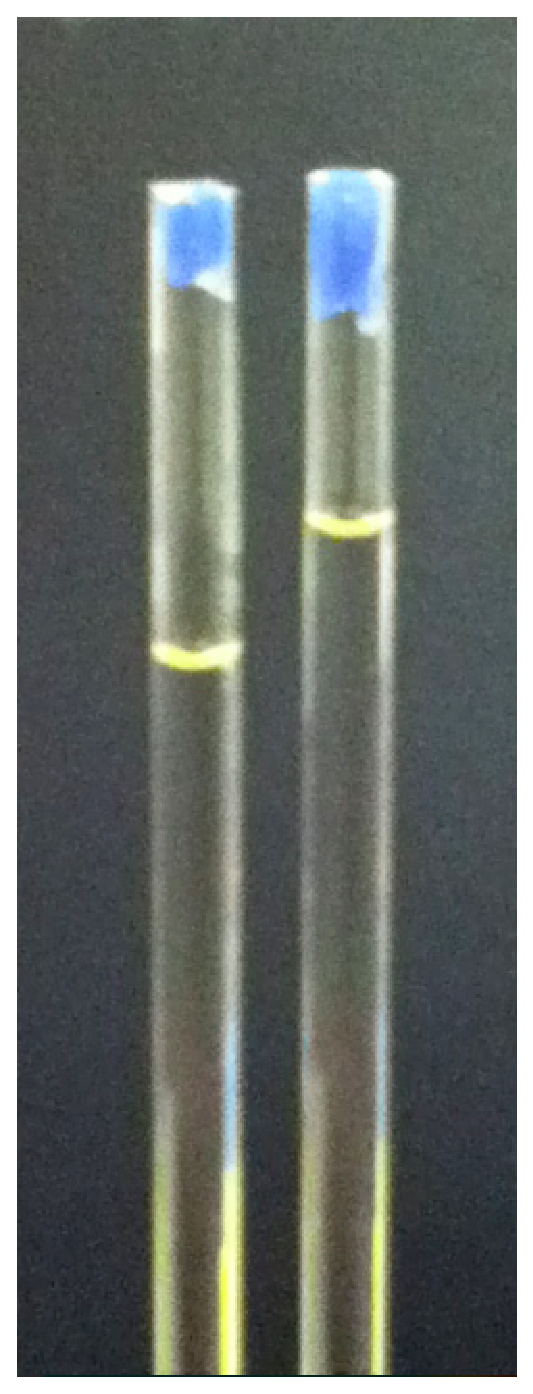
\includegraphics[width=1in]{phantom/images/tube_sealings/machinable_wax.eps}}}
%     \centerline{\emph{(c) Machinable wax}}
%   \end{minipage}\medskip
%   \begin{minipage}[t]{1in}
%     \centering
%     \centerline{\mbox{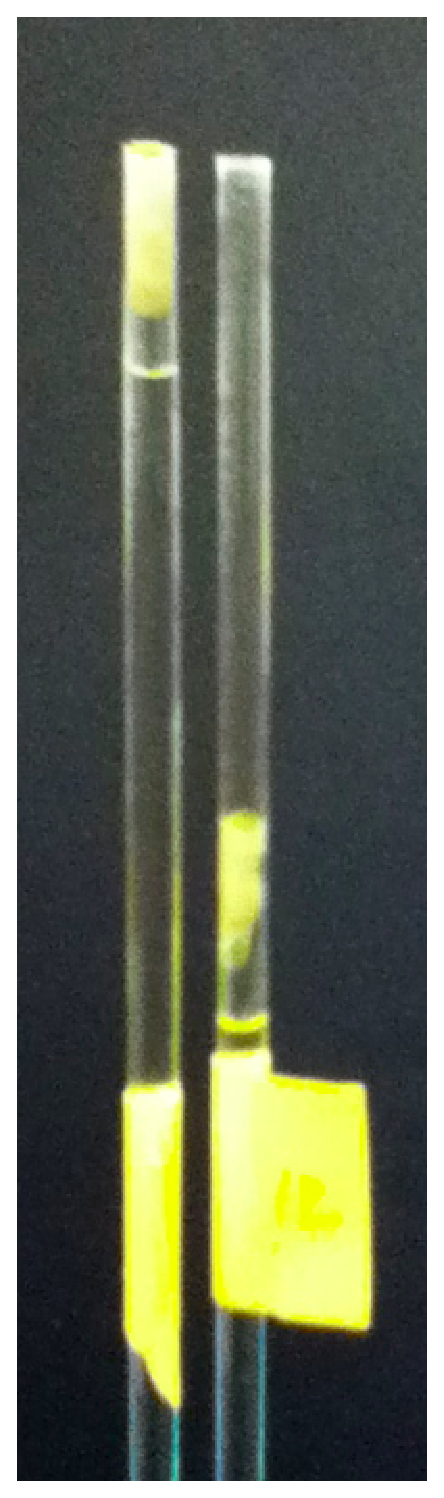
\includegraphics[width=1in]{phantom/images/tube_sealings/water_weld.eps}}}
%     \centerline{\emph{(d) Water weld}}
%   \end{minipage}

%   \begin{minipage}[t]{1in}
%     \centering
%     \centerline{\mbox{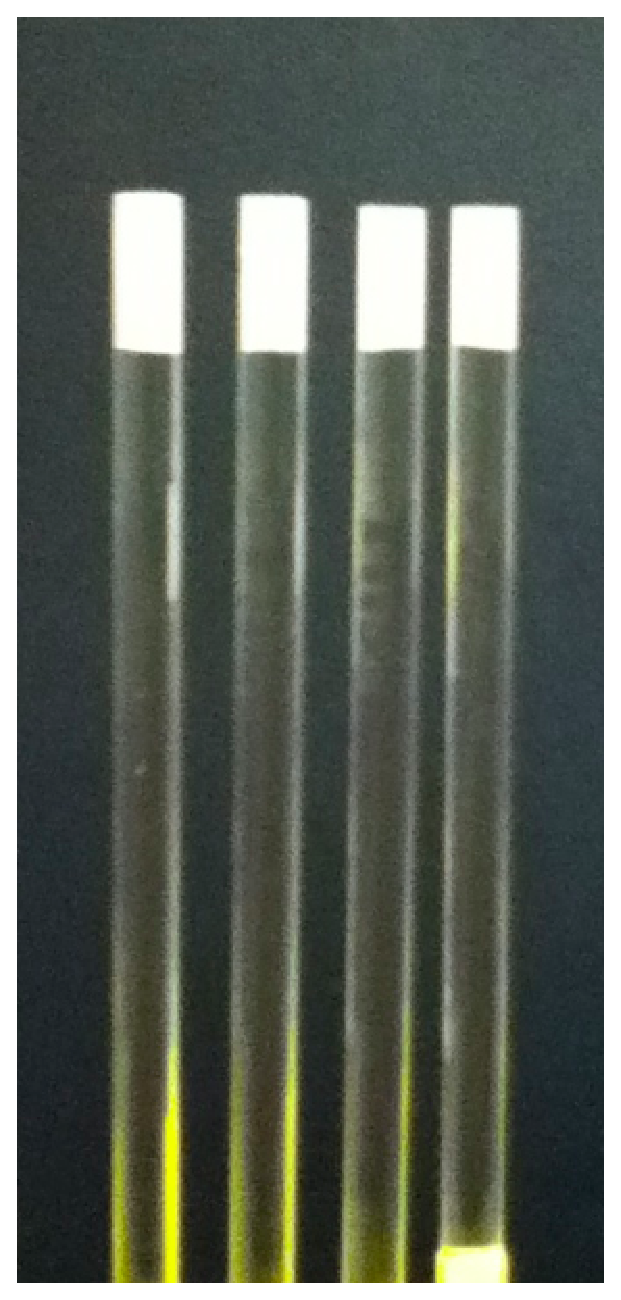
\includegraphics[width=1in]{phantom/images/tube_sealings/silicon.eps}}}
%     \centerline{\emph{(e) Silicon}}
%   \end{minipage}

% \end{figure}


\section{Installation and Use}

The new phantom is designed to rest in the head coil of a 3T MRI scanner.  It has a back plate with several
leveling screws to align the phantom in the head coil using the laser alignment system.  This alignment is
aided by alignment marks on the outside of the phantom. The phantom is then moved into the MRI scanner,
and its center is placed as close to the isocenter as possible.  While it is not required to be centered,
centering does improve the performance.  A quick alignment scan is used to ensure the phantom is in the best
location possible.  When this is done the scan is taken and processed using distortion detection and
correction software, which is not subject of the present presentation.

\section{Initial Experience}

The original phantom design, a 16-cm oil-filled cube, could not be scaled up due to weight and manufacturing
constraints. Our first modification was to look at changing the material to FR-4 since it is rigid, very flat,
and could be submerged for short periods of time to permit scanning the solid liquid interface in an MRI
machine.  Since most of the distortion is visible only in the corners, this was rapidly replaced by 8 corners
of a virtual cube, which could be connected by a rigid frame.  The weight of a tank to submerge either of
these designs to allow scanning was prohibitive, requiring a complete redesign.

\section{Conclusion}

A new phantom for the measurement and correction of nonlinear gradient field distortion of MRI systems is
presented.  It is lighter, more economic, and allows for both more accurate measurement of field distortion
and the location of the isocenter. 

\Chapter{Gradient Isocenter Localization}
\label{iso_center}
\section{Introduction}
\label{Introduction}
%The isocenter of the magnetic gradient fields inside a Magnetic Resonance (MR) Imaging scanner is used in many distortion correction methods for MR images~\cite{Dor05,LSS06a,LSS06b,LSS08a,tlee_iaeng,simple_approach,Wang04a,Wang04b}.  Currently there is no known method for estimating the gradient isocenter. All existing estimation methods are using the DICOM patient center which is very close but not exactly the same as isocenter. The different between isocenter and DICOM patient center could contribute part of the error of overall correctness of estimation.

Magnetic resonance imaging (MRI) provides an excellent modality for distinguishing different tissues in the human body, which makes this modality essential for medical applications. MRI can also be used for treatment planning of medical procedures that require a great degree of geometrical accuracy such as  functional radiosurgery~\cite{Kond99}. Unfortunately, the accuracy of MRI for medical targeting applications is compromised by the presence of geometric distortions such as non-linearities of the magnetic gradient fields or inhomogeneities of the scanner main field ~\cite{Dor05,LSS06a,LSS06b,LSS08a,tlee_iaeng,simple_approach,Wang04a,Wang04b}. Gradient nonlinearities can cause over 2mm of distortion to the location of features in the image~\cite{tlee_iaeng,simple_approach}.

Modern MRI scanners have built-in distortion correction algorithms, that rely on knowledge of the magnetic field configuration and its distortion. Built-in algorithms, which are usually proprietary, are designed based on assumed knowledge of the geometry and location of the gradient coils. A more practical approach is to use a phantom of known geometry and to derive the distortion by analyzing the MRI images generated with such a phantom ~\cite{Dor05,LSS06a,LSS06b,LSS08a,tlee_iaeng,simple_approach,Wang04a,Wang04b}. This method has the advantage that a scanner-specific correction can be applied, which can also take into account potential changes in the gradient fields over time.

Accurate knowledge of the gradient isocenter is essential to very accurate distortion correction methods, To our knowledge, existing distortion correction algorithms, both built-in and phantom based, make the assumption that the gradient isocenter coincides with the origin of the DICOM coordinates. This assumption may not be accurate and should not be used if a high degree of accuracy is necessary.

The goal of this work was to develop and implement a numerical software-based method to estimate the gradient isocenter of the magnetic field inside an MRI scanner using the MRI scan of a custom-built phantom.  In our previous work~\cite{LSS06a,LSS06b,LSS08a,tlee_iaeng}, we used an oil filled plexiglass cube with
159.50mm $\times$ 159.70mm $\times$ 158.11mm dimension that was designed to fit MR scanners that were available at that time.  Current MRI scanners have a significantly wider aperture, which necessitates a larger phantom to characterize the field distortion.  Furthermore, since the lower part of the scanner aperture is occupied by the scanner table, the scanning area occupied by the phantom or the patient is not centered on the gradient isocenter, making correction methods that assume that the phantom is centered with respect to the gradient isocenter~\cite{LSS06a,LSS06b,LSS08a,tlee_iaeng,simple_approach} obsolete and potentially inaccurate.

\section{Distortion Phantom}
A new phantom design was developed with the intention to probe the distortion in the 50 cm field-of-view (FOV) of a modern 3T MRI scanner (Magnetom Trio, Siemens).  Due to the geometry of the gradient field nonlinearity, the distortion is largest in the outer fringes of the FOV~\cite{LSS06a,LSS06b,LSS08a,tlee_iaeng}. Capturing distortion data in the periphery of the FOV is important for better accuracy of the distortion correction. Building a very large cubical oil-filled phantom is a challenge due to weight limitations and limited capability to accurately machine a very large flat surface. Thus it was felt to be impractical to simply scale up the original phantom.  Another limitation is that the phantom needs to fit inside the scanner head coil which needs to be used to achieve a sufficiently high signal-to-noise ratio.  To meet all requirements, we designed a phantom that is comprised of 64 NMR glass tubes of 3 mm inner diameter, filled with copper sulfate and arranged in 8 surfaces forming an octagon.  A water-filled cylinder in the middle of the octagon ensures a good signal generated by the tubes.  The distance between tubes on the opposite side of the surface is 205mm, which is about 28\% wider than the original phantom. In addition we also added four more surfaces to provide data and better fit the headcoil.  There are 8 removable tubes on each surface with 10 mm gap between adjacent tubes.  Each tube is about 207 mm long, which is also an increase of about 28\% in length from the original phantom.  Tubes are placed along the main axis of the magnetic $B_0$  field to reduce the effects of chemical shift and magnetic susceptibility and
resulting in high-quality axial images.

\section{Computational Algorithm}

The algorithm we described here is using simulated data set that is based the
geometric property of the phantom and the properties of the MR images.
The MR images we are using have 1mm per pixel resolution for every image and
1mm thickness between two adjacent planes. In the simulation, we will be using millimeters as unit for
each data point. Since the images we are using to collect data points are all axial scans,
we will only add noise to x and y coordinate of each data point.

\section{Tube Modeling}

The tubes are 203 mm long. So our simulation data is ranging from -100 to 100 on z axis for each tube.
The arrangement of the tubes could be seen in Figure~\ref{fig:1}.
Our algorithm is based on two standard assumptions~\cite{LSS06a,LSS06b,LSS08a,tlee_iaeng,simple_approach}.: (1) the distortion in MR images are only caused by the magnetic field inside MRI scanner and (2) the magnetic field can be perfectly described using the sum of spherical harmonic.

\begin{figure}[htb]

  \begin{minipage}[b]{2.2in}
    \centering
    \centerline{\mbox{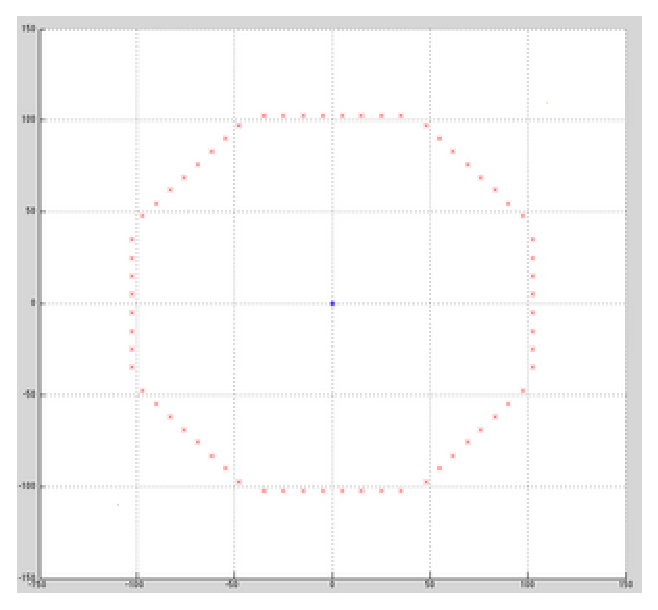
\includegraphics[width=2.2in]{isocenter/images/simulation/axial_no_distortion.eps}}}
    \centerline{\emph{(a) Axial view.}}
  \end{minipage}
  \hfill
  \begin{minipage}[b]{2.2in}
    \centering
    \centerline{\mbox{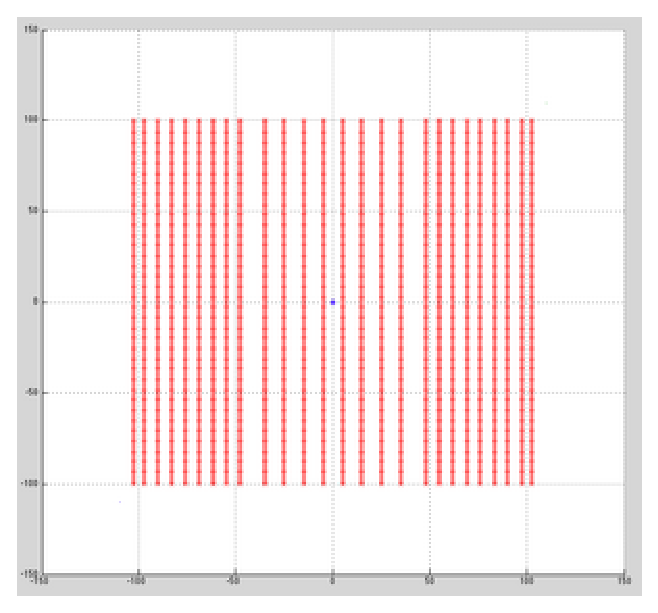
\includegraphics[width=2.2in]{isocenter/images/simulation/coronal_no_distortion.eps}}}
    \centerline{\emph{(b) Coronal view.}}
  \end{minipage}
%\hfill
%
  \caption{Phantom modeling without distortion} 
  \label{fig:1}
%
\end{figure}

The spacial coordinate of the phantom must be transformed into a coordinate relative to the gradient isocenter
of the magnetic field, see Equation~\ref{eq1}, then using the first 5 terms of the spherical harmonic we can estimate
a offset in $x$, $y$, $z$ direction, see Equation~\ref{eq2}. Finally this offset is added the original coordinate
to create a distorted model, see Equation~\ref{eq3}.  Also a very key requirement for this algorithm is that the z-axis the phantom which is parallel to the tubes must be aligned with the z-axis of the magnetic field.

\begin{eqnarray}
\begin{bmatrix}
x^\prime  \\
y^\prime  \\
z^\prime  \\
\end{bmatrix}
& = &
\begin{bmatrix}
x \\
y \\
z \\
\end{bmatrix}
-
\begin{bmatrix}
x_{iso} \\
y_{iso} \\
z_{iso}\\
\end{bmatrix}
\label{eq1}
\\
K & = &
\begin{bmatrix}
K_{x_0} \; K_{x_1} \; K_{x_2} \; K_{x_3} \; K_{x_4} \\
K_{y_0} \; K_{y_1} \; K_{y_2} \; K_{y_3} \; K_{y_4} \\
K_{z_0} \; K_{z_1} \; K_{z_2} \; K_{z_3} \; K_{z_4} \\
\end{bmatrix}
\\
\begin{bmatrix}
\alpha \\
\beta \\
\zeta \\
\end{bmatrix}
& = &
K
\begin{bmatrix}
{x^\prime}^2 + {y^\prime}^2 \\
{z^\prime}^2 \\
{z^\prime}^2 {({x^\prime}^2 + {y^\prime}^2)}^2 \\
{({x^\prime}^2 + {y^\prime}^2)}^2 \\
{z^\prime}^4 \\
\end{bmatrix}
\end{eqnarray}
\begin{eqnarray}
\begin{bmatrix}
  \Delta x \\
  \Delta y \\
  \Delta z \\
\end{bmatrix}
& = &
\begin{bmatrix}
x^\prime \alpha \\
y^\prime \beta \\
z^\prime \zeta \\
\end{bmatrix}
\label{eq2}
\\
\begin{bmatrix}
\bar{x} \\
\bar{y} \\
\bar{z} \\
\end{bmatrix}
& = &
\begin{bmatrix}
x + \Delta x \\
y + \Delta y \\
z + \Delta z \\
\end{bmatrix}
\label{eq3}
  % \bar{\alpha_i} & = & \alpha_i \left(1+  K_{\alpha_0} \left((x_i - ISO_x)^2 + (y_i - ISO_y)^2 \right)  \right. \nonumber\\
  % &&\qquad      \left.    + K_{\alpha_1}(z_i - ISO_z)^2 \right. \nonumber\\
  % &&\qquad      \left.    + K_{\alpha_2}(z_i - ISO_z)^2 \left((x_i - ISO_x)^2 + (y_i - ISO_y)^2 \right)  \right. \nonumber\\
  % &&\qquad      \left.    + K_{\alpha_3} \left((x_i - ISO_x)^2 + (y_i - ISO_y)^2 \right)^2 \right. \nonumber\\
  % &&\qquad      \left.    + K_{\alpha_4}(z_i - ISO_z)^4 \right)
% \label{eq6}
\end{eqnarray}

\section{ISO-Center Coordinate Estimation}

Using a exaggerated distortion parameter we can visualize the shape of the distortion model. Without distortion, the phantom appears as in Figure~\ref{fig:1}.  With large distortions, the phantom appears as in Figure~\ref{fig:2}, which is useful to understand the form of the distortions.  A more realistic distortion can be seen in Figure~\ref{fig:3}, which uses distortion parameters from~\cite{tlee_iaeng}.


\begin{figure}[htb]

  \begin{minipage}[b]{1.65in}
    \centering
    \centerline{\mbox{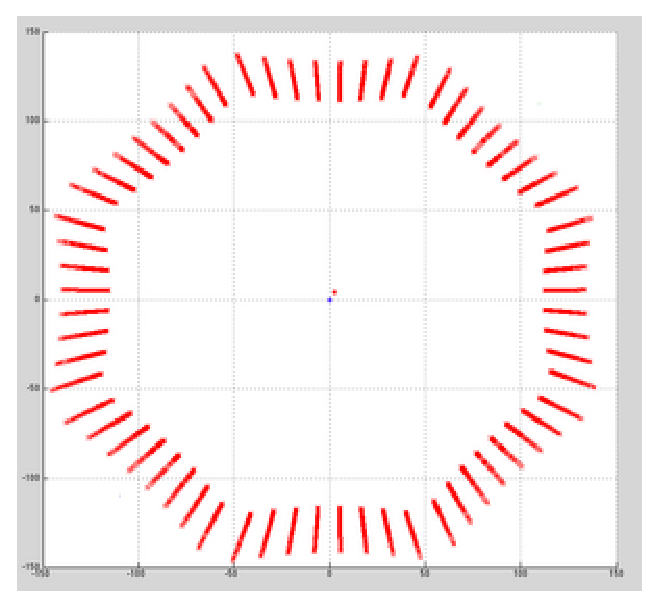
\includegraphics[width=1.65in]{isocenter/images/simulation/axial_distortion_0.eps}}}
    \centerline{\emph{(a) Axial view.}}\medskip
  \end{minipage}
  \hfill
  \begin{minipage}[b]{1.65in}
    \centering
    \centerline{\mbox{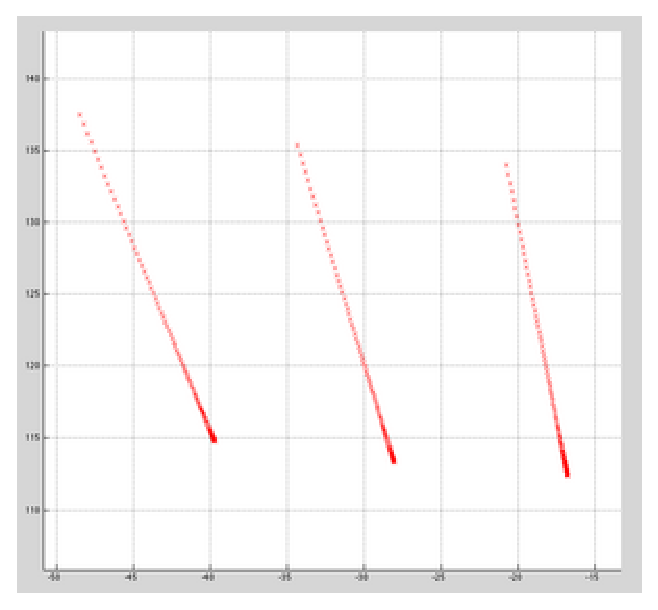
\includegraphics[width=1.65in]{isocenter/images/simulation/axial_tube_distortion_0.eps}}}
    \centerline{\emph{(b) Enlarged axial view.}}\medskip
  \end{minipage}
  \hfill
  \begin{minipage}[b]{1.65in}
    \centering
    \centerline{\mbox{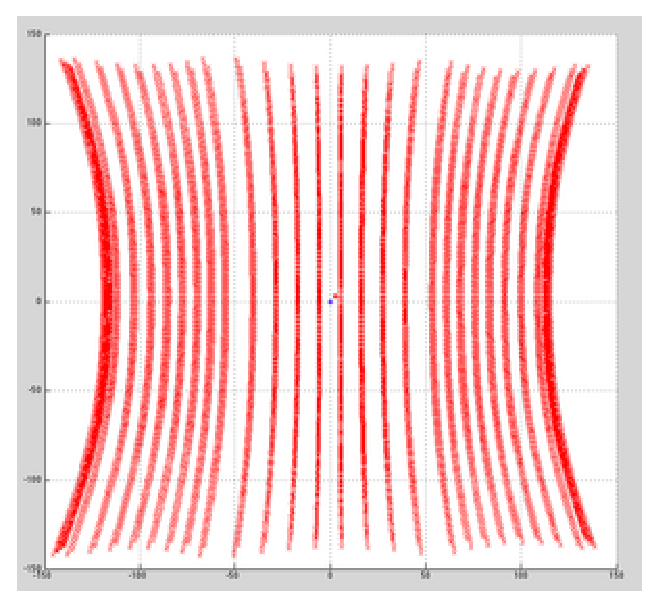
\includegraphics[width=1.65in]{isocenter/images/simulation/coronal_distortion_0.eps}}}
    \centerline{\emph{(c) Coronal view.}}\medskip
  \end{minipage}
%\hfill
%
  \caption{Phantom modeling with large distortions}
  \label{fig:2}
%
\end{figure}

\begin{figure}[htb]

  \begin{minipage}[b]{1.65in}
    \centering
    \centerline{\mbox{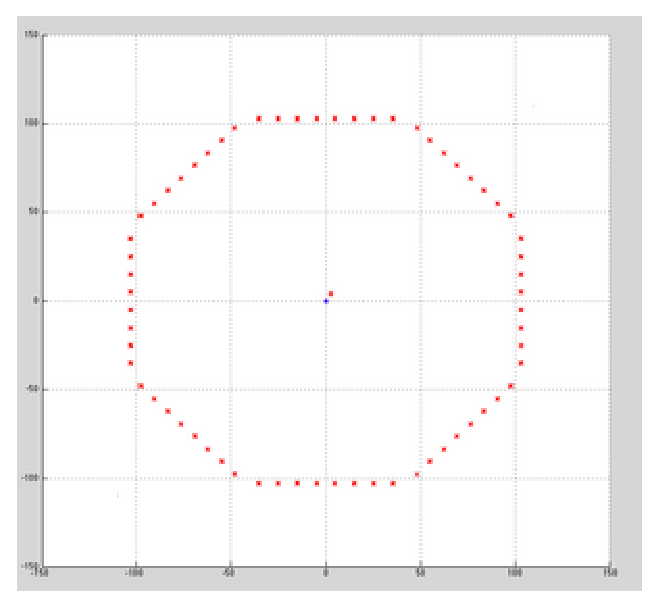
\includegraphics[width=1.65in]{isocenter/images/simulation/axial_distortion_1.eps}}}
    \centerline{\emph{(a) Axial view.}}
  \end{minipage}
  \hfill
  \begin{minipage}[b]{1.65in}
    \centering
    \centerline{\mbox{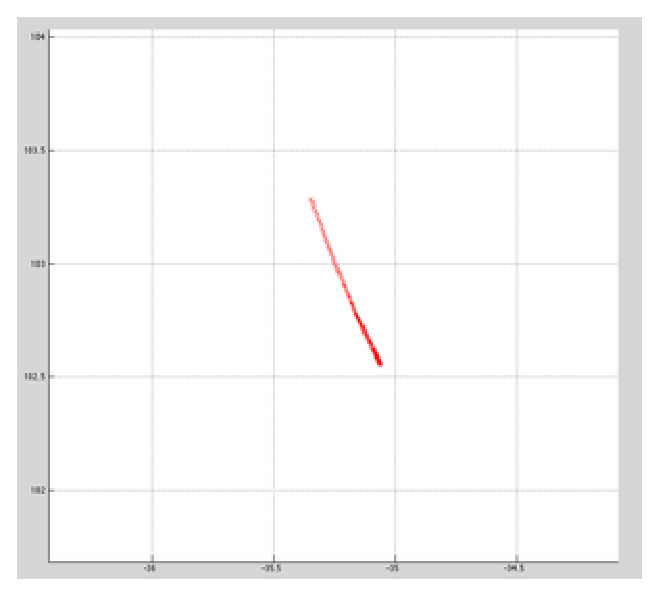
\includegraphics[width=1.65in]{isocenter/images/simulation/axial_tube_distortion_1.eps}}}
    \centerline{\emph{(b) Enlarged axial view.}}
  \end{minipage}
  \hfill
  \begin{minipage}[b]{1.65in}
    \centering
    \centerline{\mbox{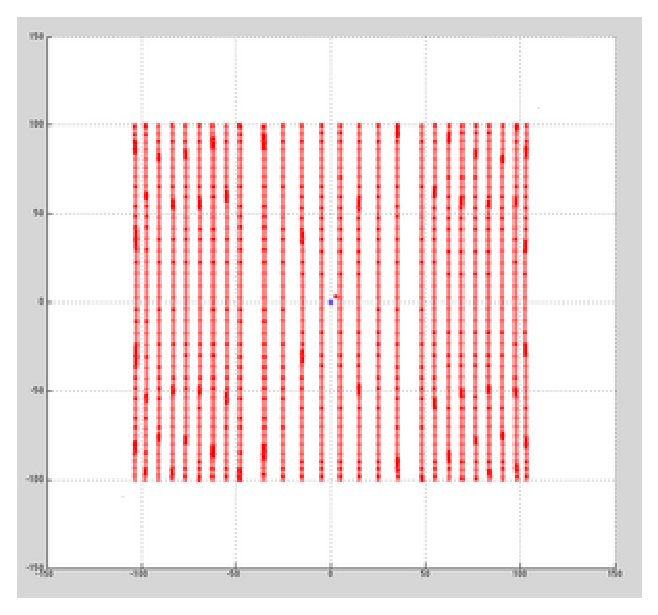
\includegraphics[width=1.65in]{isocenter/images/simulation/coronal_distortion_1.eps}}}
    \centerline{\emph{(c) Coronal view.}}
  \end{minipage}
%\hfill
%
  \caption{Phantom modeling with small distortions}
  \label{fig:3}
%
\end{figure}



Distortion in the sum of spherical harmonics is coupled in the x and y directions (orthogonal to axis), making the z axis independent.  Noise and distortion are thus very different in the z direction as opposed to the x-y plane.  We break down the gradient isocenter coordinate estimation into two big steps: estimation of z coordinate and estimation of x,y coordinate.

\subsubsection{Z-Coordinate Estimation}

Since the distortion model is based on sum of spherical harmonics, the shape of the distorted data for each tube is an even polynomial function. Figure~\ref{fig:3} shows that the realistic distortion is quite small, being about a maximum of 2 pixels, and the smaller the distortion the more sensitive the problem becomes.  With the first four terms of sum of spherical harmonics, the shape of the each tube can be seen as part of a polynomial function of 4th degree. Since the data points of tubes only represent the middle section of the 4th degree polynomial function, it is also very similar to a shape of quadratic function.  The offset between the largest distortion and the smallest distortion can be as small as 1mm.  With such a small margin, it is more practical to fit the data points to simpler model than a 4th degree polynomial.  Only the first spherical harmonic is needed in order to estimate the point where gradient is zero to measure the isocenter.  Furthermore, the first term of the sum of spherical harmonics has the largest signal to noise ratio, so we use a quadratic model to fit the data points.

We can see the distorted tube models' middle part is bending toward the center with both end bending outward.
If we were to fit each tubes to a parabola and locate the point where its gradient is zero, that point's
z-coordinate should be the same as the z-coordinate of the gradient isocenter of the magnetic field.  The z-coordinate is measured for all 64 tubes and the result averaged.  The resulting estimation is within $0.1$ mm of the actual z-coordinate.

\subsubsection{X,Y Coordinate Estimation}

The estimation of the x and y coordinates of the isocenter is the more difficult problem.
We are assuming that the difference between the distortion on x and y direction are so small that we can
treat them as if they are the same.  When this is not true, the errors on the isocenter location will be asymmetric, and it will be even more important to maintain a good numerical method to estimate the isocenter.  With that in mind, the distorted data of a tube should all stay on a plane which isocenter is also in. The intersection of such planes from each tube should be a line that
goes through isocenter. Using the isocenter estimated from previous step we should obtain an estimation
of x and y coordinate.

Since the tubes were aligned to the z-axis to reduce magnetic field distortion by the tubes, the range of data in the z-direction is of necessity larger.  In the x-y plane the range of points is controlled by the distortion, and is thus only a few pixels.  The resulting equations are highly sensitive, requiring careful handling in our numerical algorithm.

The equation of a plane in three dimensions is as follows.
\begin{eqnarray}
ax + by + cz + d & = & 0 \label{eq:plane}
\end{eqnarray}

Rewriting eq~\ref{eq:plane} with the measured data, we can solve for the plane each tube lies in.  This in turn can be used to find the intersection of the planes, which is the isocenter.
\begin{eqnarray}
-\frac{b}{a}y - \frac{c}{a}z - \frac{d}{a} & = & x \label{eq:x_orient}\\
\begin{bmatrix}
  y_0  & z_0 & 1 \\
  \vdots & \vdots & \vdots \\
  y_n & z_n & 1 \\
\end{bmatrix}
\begin{bmatrix}
-b/a\\
-c/a\\
-d/a
\end{bmatrix}
& = &
\begin{bmatrix}
x_0 \\
\vdots\\
x_n
\end{bmatrix} \nonumber\\
-m_x & = & \frac{b}{a} \nonumber\\
 k_x & = & - \frac{c}{a}z_{iso} - \frac{d}{a} \nonumber\\
  x  & = & -m_x y + k_x \nonumber\\
\begin{bmatrix}
1 \; m_x
\end{bmatrix}
\begin{bmatrix}
x \\
y
\end{bmatrix}
& = &
k_x \label{eq:x_est}
\end{eqnarray}

Note that eq~\ref{eq:plane} can be rewritten so either x or y is independent, which affects the error in standard least squares.  This becomes particularly important when the non-linearity is not the same in the x and y directions, as scaling is also well known to cause problems for least squares.
\begin{eqnarray}
-\frac{a}{b}y - \frac{c}{b}z - \frac{d}{b} & = & y \label{eq:y_orient}\\
\begin{bmatrix}
  x_0  & z_0 & 1 \\
  \vdots & \vdots & \vdots \\
  x_n & z_n & 1 \\
\end{bmatrix}
\begin{bmatrix}
-a/b\\
-c/b\\
-d/b
\end{bmatrix}
& = &
\begin{bmatrix}
y_0 \\
\vdots\\
y_n
\end{bmatrix} \nonumber\\
-m_y & = & \frac{a}{b} \nonumber\\
 k_y & = & - \frac{c}{b}z_{iso} - \frac{d}{b} \nonumber\\
  y  & = & -m_y x + k_y \\
\begin{bmatrix}
1 \; m_y
\end{bmatrix}
\begin{bmatrix}
y \\
x
\end{bmatrix}
& = &
k_y \label{eq:y_est}
\end{eqnarray}


% \begin{eqnarray}
% -\frac{a}{b}y - \frac{c}{b}z - \frac{d}{b} & = & y
% \end{eqnarray}

As we can see from figure~\ref{fig:4}, by using equation~\ref{eq:x_orient} and equation~\ref{eq:y_orient} to estimate
planes in figure~\ref{fig:4}(b) and \ref{fig:4}(d) respectively we get and quite accurate x and y coordinate
estimate. However, when you swap the choice of equations, even though they are mathematically identical,
they make a huge numeric difference as shown in \ref{fig:4}(a) and \ref{fig:4}(b).

\begin{figure}[htb]

  \begin{minipage}[b]{0.48\linewidth}
    \centering
    \centerline{\mbox{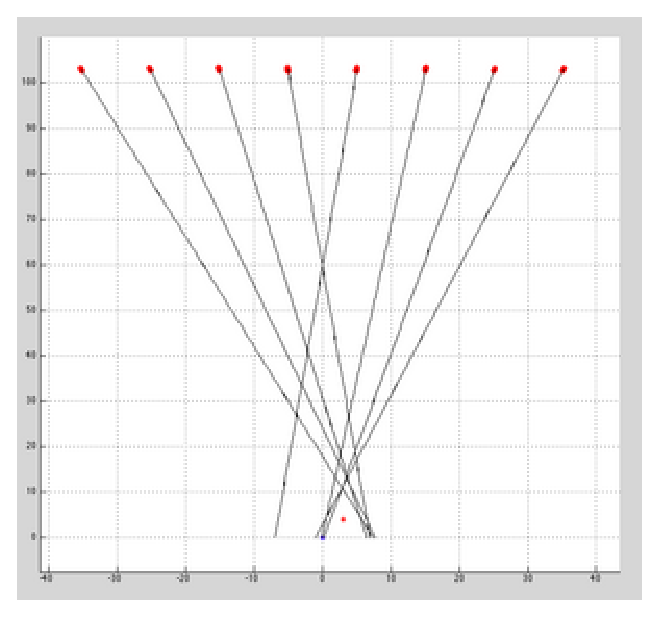
\includegraphics[width=1.65in]{isocenter/images/simulation/tube_plane_large_error_y.eps}}}
    \centerline{\emph{(a) LS fit with y orientation.}}\medskip
  \end{minipage}
  \hfill
  \begin{minipage}[b]{0.48\linewidth}
    \centering
    \centerline{\mbox{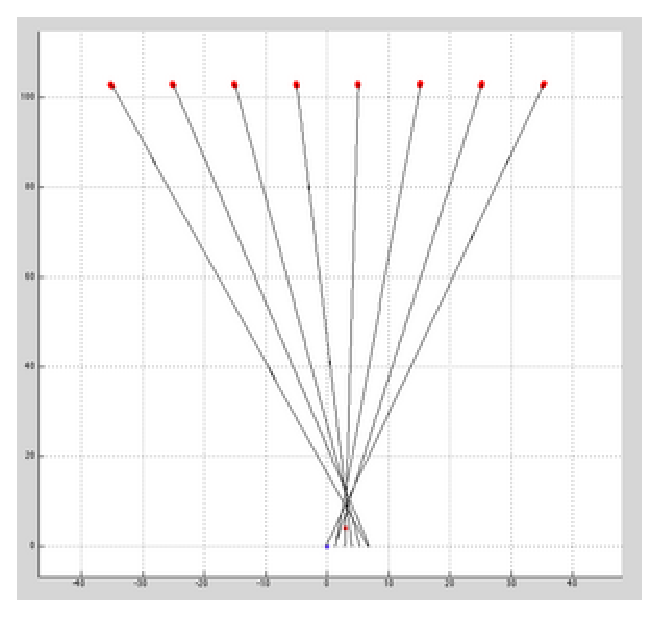
\includegraphics[width=1.65in]{isocenter/images/simulation/tube_plane_small_error_x.eps}}}
    \centerline{\emph{(b) LS fit with x orientation.}}\medskip
  \end{minipage}
  \begin{minipage}[b]{0.48\linewidth}
    \centering
    \centerline{\mbox{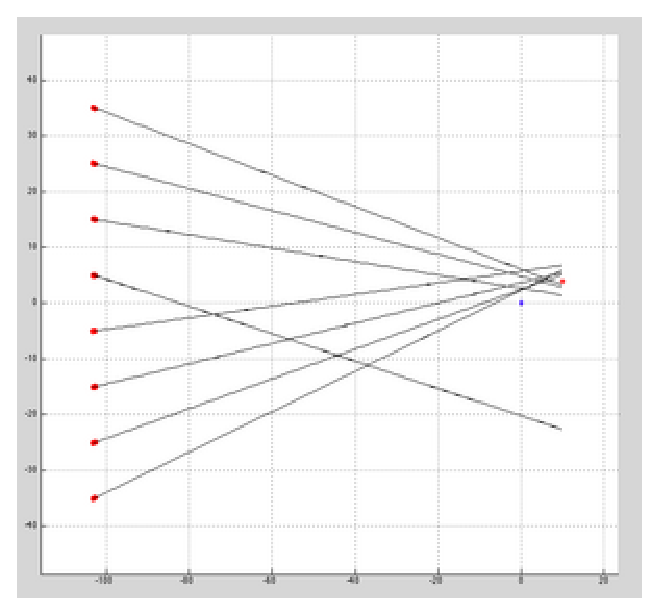
\includegraphics[width=1.65in]{isocenter/images/simulation/tube_plane_large_error_x.eps}}}
    \centerline{\emph{(c) LS fit with x orientation.}}\medskip
  \end{minipage}
  \hfill
  \begin{minipage}[b]{0.48\linewidth}
    \centering
    \centerline{\mbox{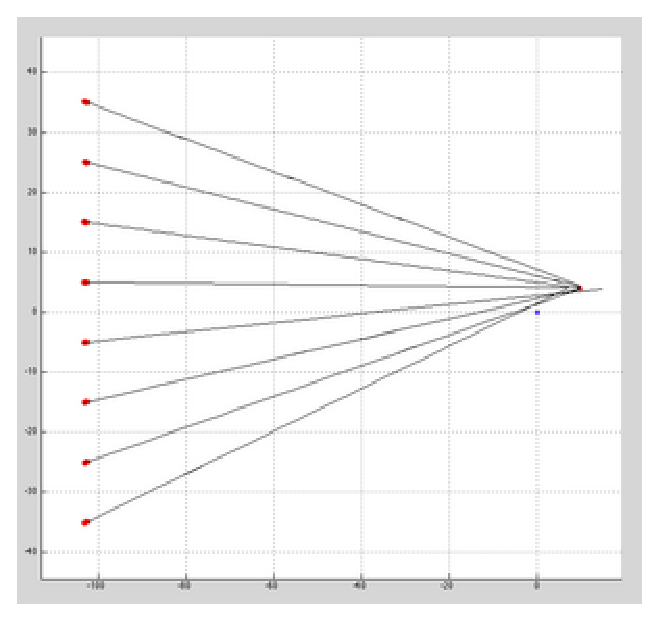
\includegraphics[width=1.65in]{isocenter/images/simulation/tube_plane_small_error_y.eps}}}
    \centerline{\emph{(d) LS fit with y orientation.}}\medskip
  \end{minipage}
  \caption{Phantom modeling with distortion, showing differences in isocenter estimates due to how the LS equation is oriented.} 
  \label{fig:4}
%
\end{figure}

When estimating the x-y coordinate using least square we should keep in mind that least square assumes
there is no observation error, it will only try to correct one side of the equation depending on how it
is setup. With this in mind, we uses equation \ref{eq:x_est} for x coordinate estimation and \ref{eq:y_est}
for y estimation. For the tubes on the diagonal planes, as we can see in fig\ref{fig:diagonal},
they offers neither a good data for x nor y coordinate estimation as compared to fig~\ref{fig:4} (b) and (d). So in order to utilize the diagonal
tubes we have to rotate these tubes to either x or y plane, and get an estimation of a rotated x-y
coordinate, then rotate the rotated x-y coordinate back and average it with original x-y coordinate
estimation.

\begin{figure}[htb]

  \begin{minipage}[b]{0.48\linewidth}
    \centering
    \centerline{\mbox{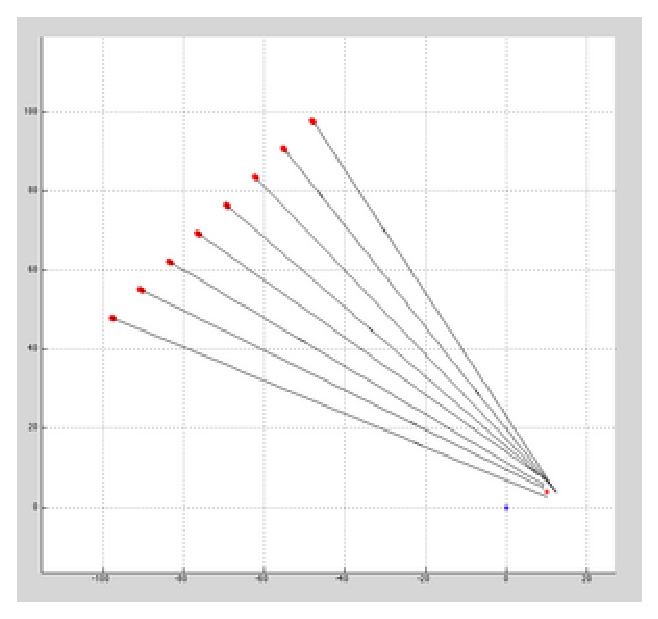
\includegraphics[width=1.65in]{isocenter/images/simulation/tube_plane_diagonal_using_x.eps}}}
    \centerline{\emph{(a) LS using x orientation.}}\medskip
  \end{minipage}
  \hfill
  \begin{minipage}[b]{0.48\linewidth}
    \centering
    \centerline{\mbox{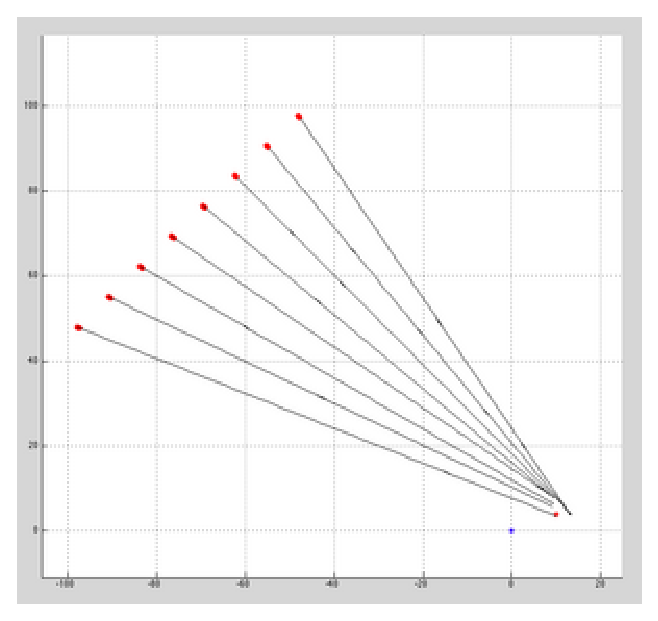
\includegraphics[width=1.65in]{isocenter/images/simulation/tube_plane_diagonal_using_y.eps}}}
    \centerline{\emph{(b) LS using y orientation.}}\medskip
  \end{minipage}
  \caption{Phantom modeling with distortion, showing how diagonal tube planes without rotation do not improve the estimates produced.} 
  \label{fig:diagonal}
%
\end{figure}

In order to obtain a good estimate, we thus must separate the estimation of x and y, as well as rotate the diagonal oriented tube planes and then separate the estimation of x and y and rotate back.  We refer to this algorithm as Rotated
Separable Least Squares (RSLS). We now present the RSLS algorithm to estimate x-y coordinate of gradient isocenter as follows:

\begin{enumerate}
\item Use equation~\ref{eq:x_orient} to estimate tube planes for tubes at upper and lower surfaces.
\item Solve equation~\ref{eq:x_est} for x and y, but only use x for x coordinate.
\item Use equation~\ref{eq:y_orient} to estimate tube planes for tubes at left and right surfaces.
\item Solve equation~\ref{eq:y_est} for y and x, but only use y for y coordinate.
\item Rotate diagonal tubes $\pi/4$, and repeat steps 1-4.
\item Rotate x-y coordinate obtained from previous step by $-\pi/4$.
\item Average the x-y coordinate from previous step with x-y coordinate calculated from step 2 and step 4 for final x-y estimation.
\end{enumerate}

Alternatively, after obtaining the plane equation parameters we can put everything into one matrix and do
a one time estimation using either least square or total least square. In table~\ref{table:symmetric}, we
can see the comparison of accuracy of estimating an isocenter at $[4 \; 4\; 3]$ using different methods.
Least square tends to lean toward one coordinate
more depends on setup, while total least square has an accurate and very balanced result due to the property
that it will try to correct errors on both side of the equation. In the contrast, our method has best
properties of both methods:

\begin{itemize}
  \item It is accurate. For both x and y coordinate it does a better job than total least square, much better than least square's worst case and very close to least square's best case.
  \item It has very balanced result. Both x and y coordinates are very close the correct result equally just like total least square.
  \item It has very tight error boundaries. After 200 runs, it's error is tighter than standard least square.
\end{itemize}

Therefore, our estimation method is a good alternative to traditional least square or total least square methods. Although it might require more computation, it could be easily dealt by modern GPU computing. And due to the fact that each least square estimation has relative small matrix, and each estimation is independent of each other, it is very close to ``embarrassingly parallel'' type of problems and makes it easy to solve.


%KES the other is too nice for all examples so we need to show the ugliness.  I don't have the data, so I am setting what
%    I recall from our talk last night.  It will need your data.

In table~\ref{table:symmetric}, the test is run using a symmetric x-y axis distortion. We can see that all three methods performed very well. RSLS method's result is slightly better than Total Least Squares (TLS), and one on y axis it is better than standard Least Squares method.

%KES - what is two LS method and what is one LS method?  must explain in text?
%      is one traditional and the other our new method?
\begin{table}
  \begin{tabular} {| l | r | r | r | r | r | r |}
    \hline
    & $\bar{x}$ & $\sigma_x$ & err & $\bar{y}$ & $\sigma_y$ & err  \\
    \hline
    RSLS  & 3.9709 & 0.1068  & 0.0291 & 3.9677 & 0.1008 & 0.0323\\
    \hline
    LS & 3.9950 & 0.1118 & 0.0050   & 3.9414 & 0.1011 & 0.0586 \\
    \hline
    TLS  & 4.0800 & 0.1035  & 0.0800   & 4.0800 & 0.0964 & 0.0800 \\
    \hline
  \end{tabular}
  \caption{Average of 200 runs using different methods for estimating the isocenter at $[4 \; 4 \; 3]$ in the presence of symmetrical distortion} 
  \label{table:symmetric}
\end{table}


When the distortion is not symmetrical the issue of proper estimation becomes crucial. In table~\ref{table:nonsymmetric}, we show the result of using non-symmetrical distortion in which the y direction was set to be twice the distortion in the x. In this test, TLS method's result is the worst, off by a few millimeters.  Both LS and RSLS show comparable degradation of performance in x.  LS shows degradation in the estimation of y as well, but RSLS, since it is separable, does not experience any degradation of it. Only the RSLS's result remains quite accurate. This shows the advantage of RSLS over the other two traditional methods.


\begin{table}
  \begin{tabular} {| l | r | r | r | r | r | r |}
    \hline
    & $\bar{x}$ & $\sigma_x$ & err & $\bar{y}$ & $\sigma_y$ & err \\
    \hline
    RSLS & 3.8073 & 0.1117 & 0.1927   & 3.9838 & 0.1059 & 0.0162 \\
    \hline
    LS  & 4.2191 & 0.1117    & 0.2191 & 3.8765 & 0.1003 & 0.1235 \\
    \hline
    TLS  & 9.5744 & 0.2616 & 5.5744   & 8.6905 & 0.2393 & 4.6905 \\
    \hline
  \end{tabular}
  \caption{Average of 200 runs using different methods for estimating the isocenter at $[4 \; 4 \; 3]$ in the presence of non-symmetrical distortion } 
  \label{table:nonsymmetric}
\end{table}


\section{Conclusion}
In this work, we developed a new numerical algorithm to accurately determine the gradient isocenter
of MRI scanners based on a new distortion correction phantom. Knowledge of the gradient isocenter is an essential part of gradient-nonlinearity correction methods.  We have shown that the method used in this work to estimate the gradient isocenter is a good alternative to more traditional estimation methods such as least squares and total least squares. The new algorithm is particularly suited when the image data are extremely sensitive to the presence of noise and asymmetric distortion. Using simulated (but realistic) distortion data, it was shown, that the resulting estimated isocenter was within $0.2$ mm of the actual gradient isocenter, leading to a better estimate than the currently used DICOM coordinate center.


\Chapter{Data Extraction}
\label{data_extraction}
\section{Introduction}
In order for our estimation to work we need to collect two different types of data for our calculations. 
One is the true geometric dimension of our phantom, the other is the corresponding distorted signal that
represent those known geometric locations inside MR images. Some of these data can be relied on manufacture's
measurement, while others would require us to extract information from various types of images to estimate the
measurements. In this chapter we will discuss how we obtain each measurements and algorithm involved in those
processes.

\section{Tubes}
\label{tubes}

\section{Water Tank}
\label{ct_tank}

\subsection{CT Scan overview, target surfaces}
\begin{figure}[htb]
  \begin{minipage}[t]{2.75in}
    \centering
    \centerline{\mbox{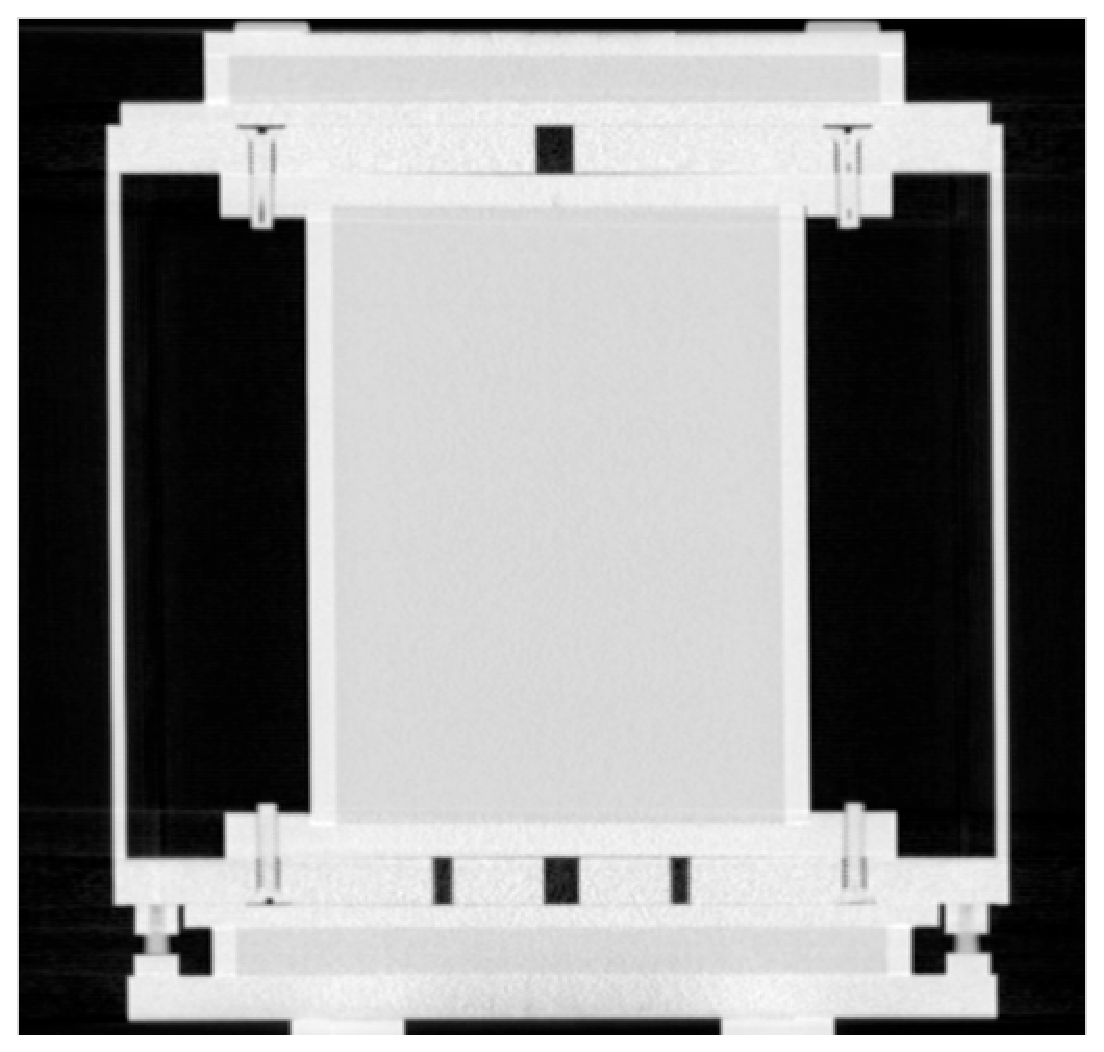
\includegraphics[width=2.75in]{data_extraction/images/ct_coronal_mid_slice.eps}}}
    \centerline{\emph{(a) Coronal view, center slice}}
  \end{minipage}\medskip
  \begin{minipage}[t]{2.75in}
    \centering
    \centerline{\mbox{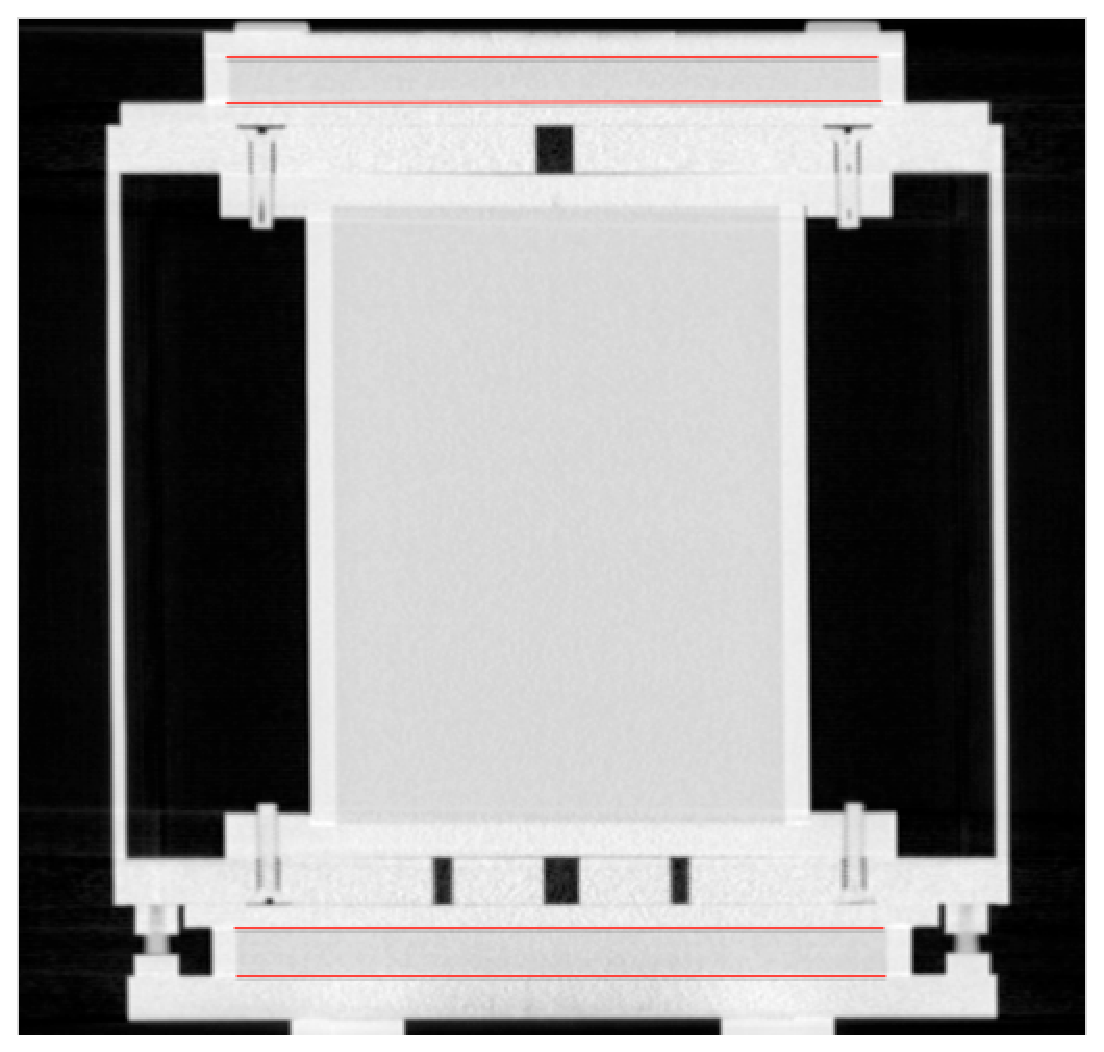
\includegraphics[width=2.75in]{data_extraction/images/ct_coronal_mid_slice_marked_surface.eps}}}
    \centerline{\emph{(b) Marked target surfaces}}
  \end{minipage}
\end{figure}

\subsection{Simple Canny}




\section{Water Tank MRI}
\label{mri_tank}

\subsection{MRI tank surface extraction}
The end tanks surfaces are very cruicial for estimating undistortion parameters. They will be used together 
with the CT tank measurements we obtained previously to do the estimation.

\subsection{extraction}
Comparing to CT images, MR images does not capture the materials of the phantom itself. It only captures 
signals generated from water and copper sulfate. However, depending on which secion of the phantom we are
looking at, there could be quite amount of noises that could be a challenge to remove. 

In the following sample MR image, we can see that top section's contrast ratio is pretty good. Not only that
we can easily identify it with our eyes, after slightly tweeking canny's algorithm, we can get a very good 
edge result. However, the bottom tank region is very noise. Although we can identify them our eye, canny
algorithm has a very hard time produce good edge result for that section. 

\begin{figure}[htb]
  \begin{minipage}[t]{2.75in}
    \centering
    \centerline{\mbox{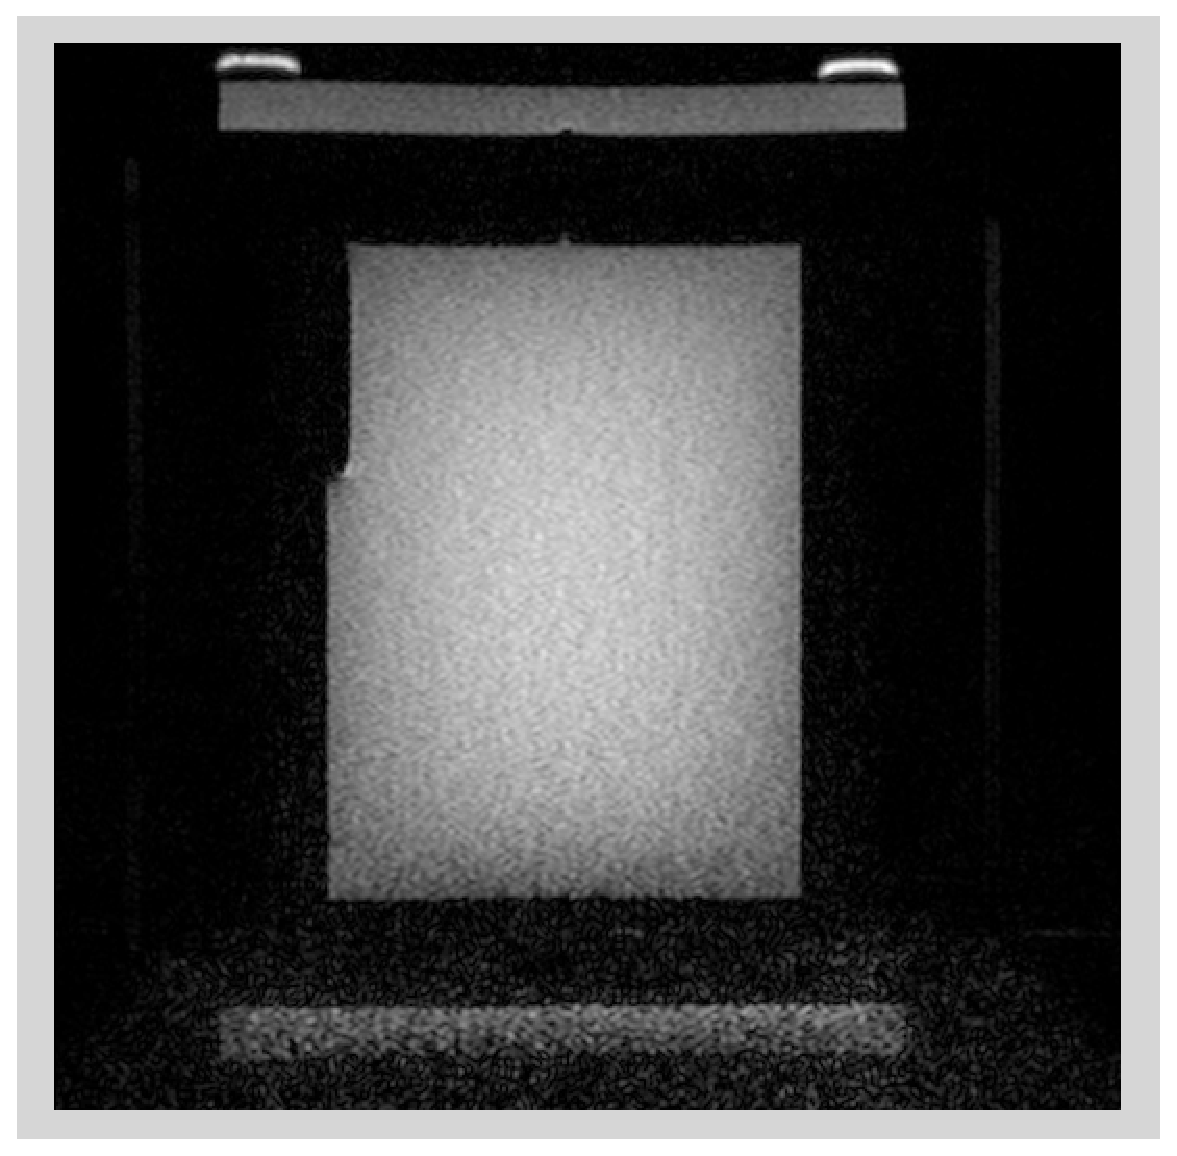
\includegraphics[width=2.75in]{data_extraction/images/MRI/mid_slice/112.eps}}}
    \centerline{\emph{(a) MR images}}
  \end{minipage}\medskip
  \begin{minipage}[t]{2.75in}
    \centering
    \centerline{\mbox{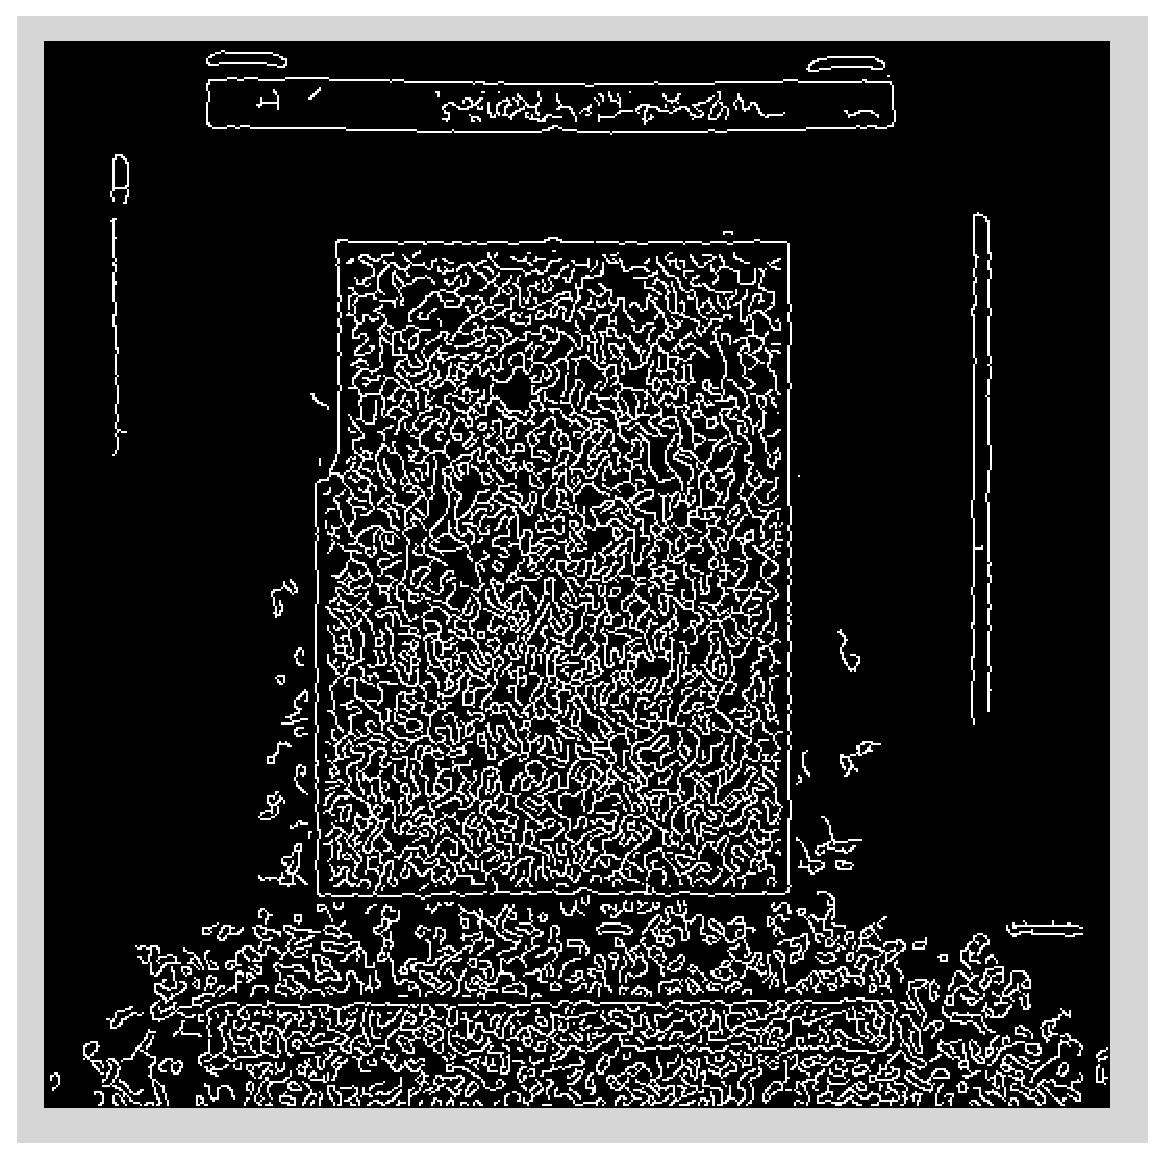
\includegraphics[width=2.75in]{data_extraction/images/MRI/mid_slice/112_canny_default.eps}}}
    \centerline{\emph{(b) Canny algorithm on (a) using default parameters}}
  \end{minipage}

  \begin{minipage}[t]{2.75in}
    \centering
    \centerline{\mbox{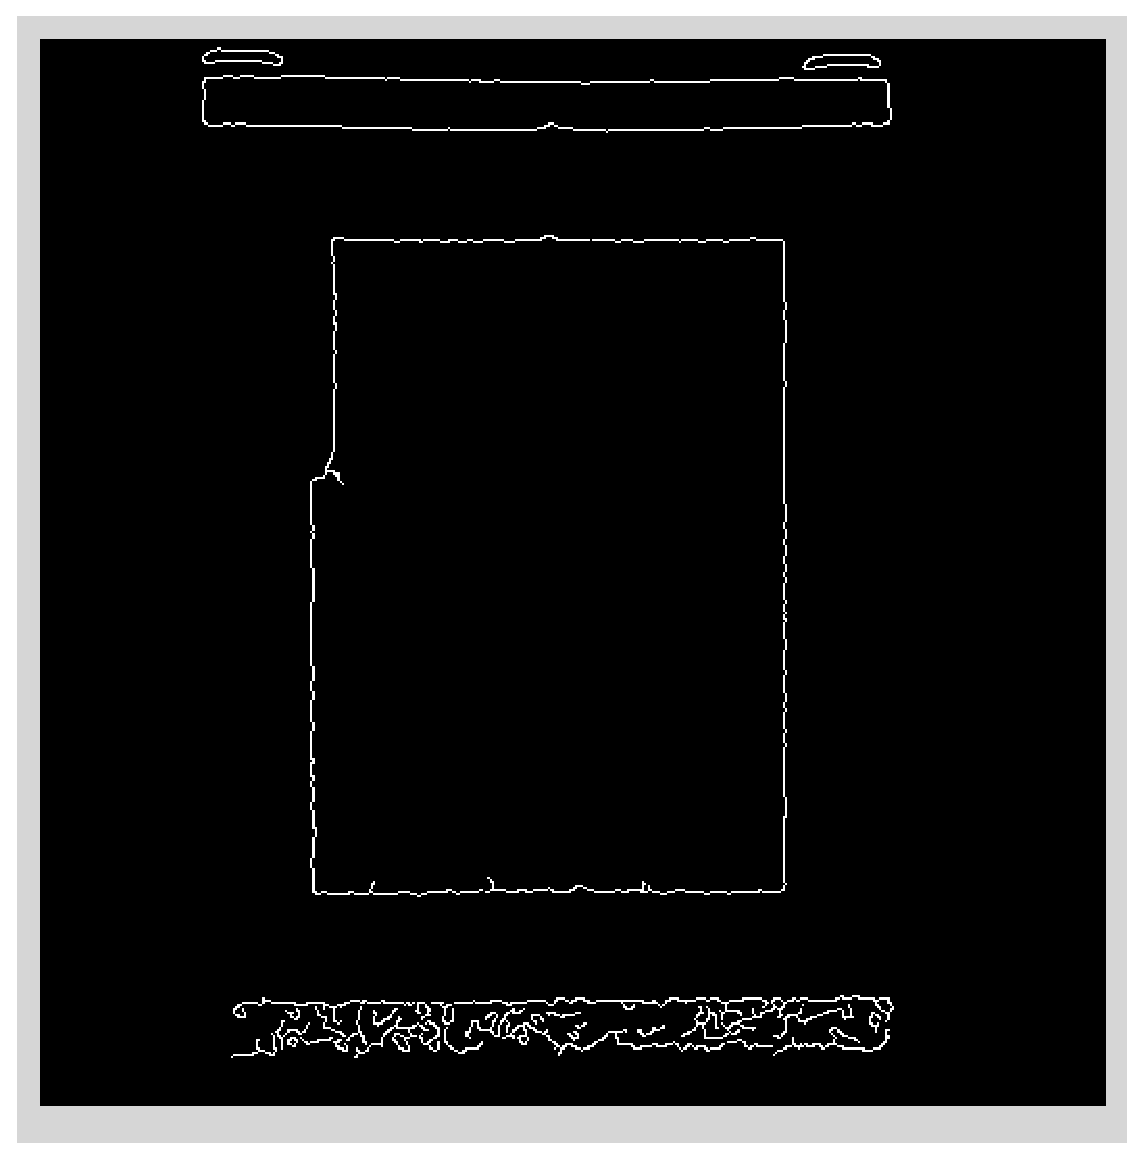
\includegraphics[width=2.75in]{data_extraction/images/MRI/mid_slice/112_canny_[0.1,0.2].eps}}}
    \centerline{\emph{(b) Canny algorithm on (a) using parameter [0.1, 0.2]}}
  \end{minipage}\medskip

  \begin{minipage}[t]{2.75in}
    \centering
    \centerline{\mbox{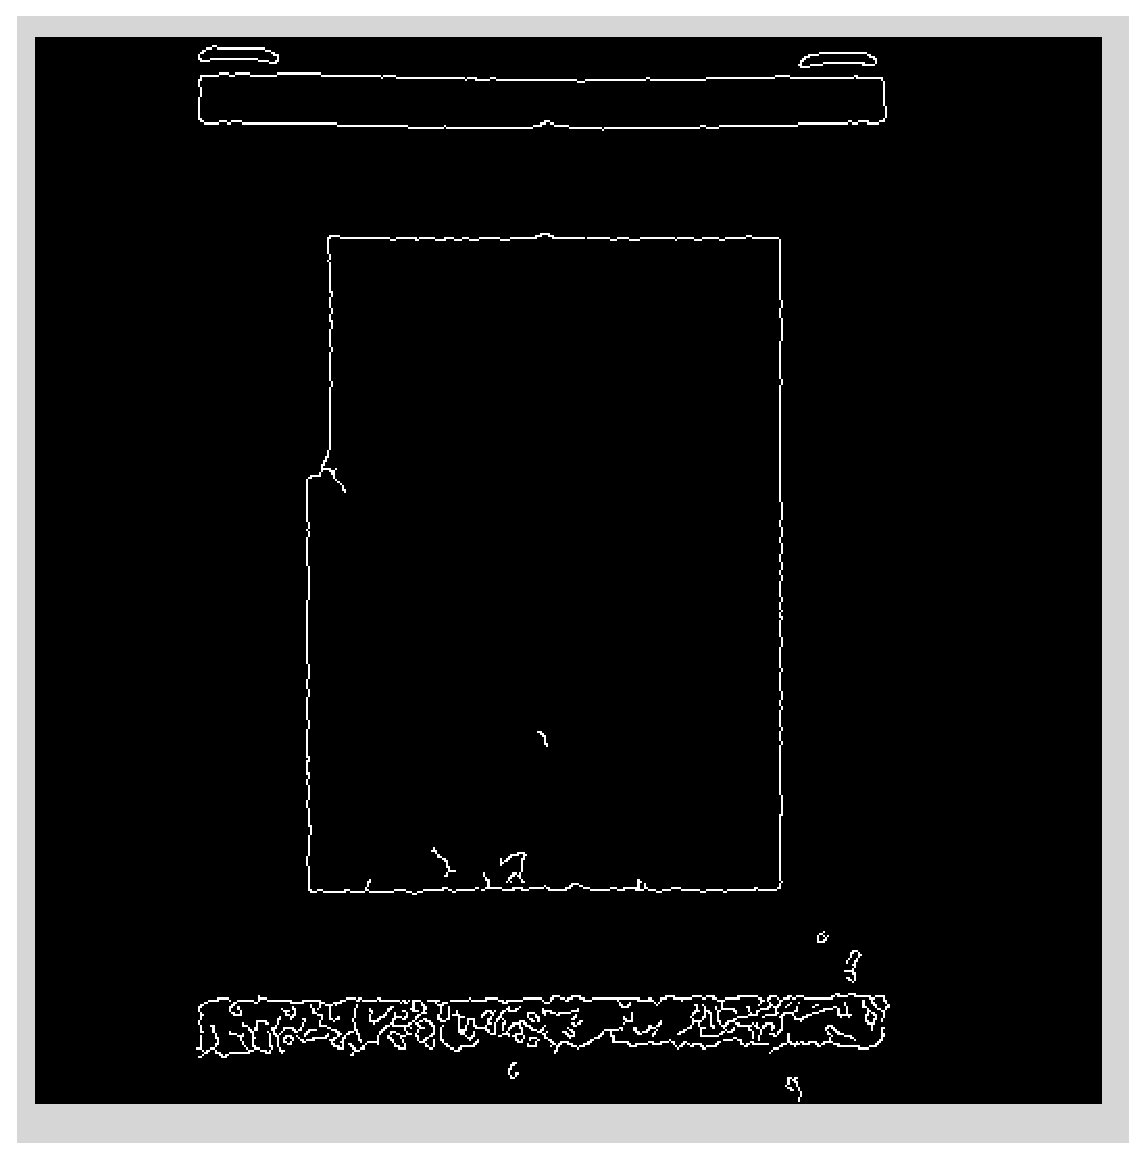
\includegraphics[width=2.75in]{data_extraction/images/MRI/mid_slice/112_canny_[0.09,0.18].eps}}}
    \centerline{\emph{(b) Canny algorithm on (a) using parameter [0.09, 0.18]}}
  \end{minipage}


\end{figure}


Since the overall layouts of tanks in MR images and CT images are quite similar -- they both have water tanks
at top and bottom of images and we are looking for top and bottom edges of those water tanks in both imagse.
So we decided that the best approach is to start with the algorithm we used in CT images even though there
are some big differences. Two big differences are:

\begin{enumerate}
  \item The surfaces we are looking for are curve due to distortion of the magnetic field.
  \item Water tanks appear in the bottom region of the images are quite noisy, by just tweeking canny's
    parameter will not give too much improvements.
\end{enumerate}

However, we believed that those issues could be overcome once we have reached the portion of algorithm that 
deal with those regions. On the bigger picture, we are still going to follow the same algorithm we used in
CT images water tank extractions:

\begin{enumerate}
  \item Use a middle slice to determine approximately where each surfaces are located, and we are going to
    used the same boundary to extract surface regions from every other images from the same image set. This 
    works because we have previously corrected any tiltness to each axis. So if a surface is in a particular
    region of one slice, we know for sure that it will be in the same region of other slices.
  \item Once we have extracted surface regions, we can determine the left and right boundaries of that surface
    by analysing the intensity histogram of each region.
  \item With each surface regions' left and right boundaries are set, we can apply our algorithms to filter out
    unwanted edges.
\end{enumerate}

\subsection{Region extraction}

One of the biggest challenge in dealing MR images is noise, especially the tank on the bottom of images. 
This water tank is sticking out of the head coil, so noises around that region is considerably larger than
other regions of the same image. Although canny algorithm does have a way to deal with noises in images by 
blurring source images, it is not enough to overcome the noises in MR images in order for us to get a very
good edge result.

Our approach is to sum previous and next slice of the imamge we are working on in order to cancel out some
noises and also enhance some features. Unlike CT images, in which flat surface will stay flat through out the
series. In MR images, due to the distortion of the magnetic field, flat surfaces will appear to be curved.
That curvature would get more and more severe toward the outer region of the phantom. This means when
overlapping previous and next images from the series to our target images, we could potentially add some 
pixels that does not belongs to the images we are processing. However, this is not a big issue for the
following reasons:

\begin{enumerate}
\item The overall distortion is quite small, the distorted outer edge of the water tank is approximately 
  3-4 pixels off the original position. This difference is spread out across 200 slices,
\item The reolution of the MR images is about 1mm, any changes smaller than 1mm won't get picked up. 
\end{enumerate}

So adding one slice before and one slice after will enhance the features we are looking for and will not 
add any unwanted features into the images.

Here is a comparison of the the histogram of before and middle column of middle slices before and after 
adding adjacent images.

% \begin{figure}[htb]
% \end{figure}

\subsection{Boundary detection}

For left and right boundary detection we are going to apply the similar method we used in CT images. 
Unlike CT images' left right boundaries, there is no phantom tank material signal in MR images, 
so we could just use maximum and minimum peak as a way to distinguish boundaries. Slices toward each end
of the phantom will have significantly more noises, they are very hard to distinguish. But if we use the same
method as we used in CT images we should have no problem detecting most boundaries which will give us more
than enough data for our estimation. This algorithm goes as follows:

\begin{enumerate}
  \item Run left-right boundary detection on the middle slice image. Due the good quality, we will get a 
    pretty accurate left and right boundary. The algorithm will not only return left and right boundary
    locations, but will also return several parameters used for tracking future boundaries.
  \item Run the algorithm two more passes, each run will take each half of the image set and iterate from
    the slice closest to mid slice to slice furthest to the mid slice. At the beginning of each run, we will
    pass the parameters we obtained from previous step.
  \item We just run this algorithm to the inside surface of exterior tank due to the fact that we had make
    sure there was no rotation and tiltness in each different axis. This means other three surfaces will
    share the left and right boundaries with exterior outside surface.
\end{enumerate}

\subsection{Noisy Edge reduction}

For noisy edge reduction, we are going to follow these steps:
\begin{enumerate}
  \item We are going to apply the short edges removal as we did in CT images. 
  \item After removing short edges, what's left are very hard to distinguish. In CT images, we knew the edges
    are supposed to be a straight line, so we filtered the noises based on a straight line model. In MR images,
    edges are distorted and are supposed to be curved. Since exterior tank gets very good signal and very good
    edge results, we can use the edge result from exterior tank's opposite surfaces' edge result as a model
    for filtering inferior tank's surface edge.
\end{enumerate}



\Chapter{Parameter Estimation}

% \Chapter{Verification}
\Chapter{Summery and Conclusion}

\bibliographystyle{plain}
\bibliography{thesis}
\end{document}
